\documentclass[aspectratio=169, 14pt]{beamer}
\usepackage{tikz}
\usepackage{subfig}
\title{Using Pseudo-Random Numbers Repeatably in a Fine-Grain Multithreaded Simulation}
\author{Dmitry Savin}
\date{\today}

\usepackage[utf8]{inputenc}

\setbeamersize{text margin left=0pt,text margin right=0pt}

\begin{document}
\begin{large}

 \frame{\titlepage}


 \begin{frame}{Motivation}
 \large
  \begin{itemize}
   \item Geant4 is a toolkit for the Monte Carlo simulation of the passage of particles through matter
   \item Monte Carlo simulation relies on pseudo-random numbers
   \item The numbers must seem uncorrelated
   \item Reproducibility from any point of simulation is needed
  \end{itemize}
 \end{frame}
 
  \begin{frame}{Motivation}
  \large
  \begin{itemize}
   \item Geant4 uses event-level parallelism
   \begin{itemize}
     \item Each event is simulated independently
     \item Independent PRNGs in a small fixed number of threads
    \end{itemize}
    $\Rightarrow$ an event is defined by the generator state at the beginning\\ \ \\
   \item GeantV uses track-level parallelism
    \begin{itemize}
     \item Similar tracks from many events are collected in "baskets"
     \item Baskets are processed in parallel to utilize vectorisation
     \item A big number of tracks is needed to reduce overhead
     \item Number of tracks, baskets and threads change during the simulation
    \end{itemize}
   $\Rightarrow$ a new mechanism is needed for reproducibility
  \end{itemize}

 \end{frame}

 
 \begin{frame}{Pedigrees}
  \begin{itemize}
   \item the rank of a track - the number of sibling tracks created by its parent track before it
   \item the pedigree of a track - the sequence of ranks of its ancestor tracks
   \item the hashed pedigree can be stored by the track and used to seed the generator
  \end{itemize}
 \end{frame}


 \begin{frame}{Merkle–Damgård hash calculation}
  \begin{figure}
   \scalebox{.5}{\setlength{\unitlength}{4144sp}%
%
\begingroup\makeatletter\ifx\SetFigFont\undefined%
\gdef\SetFigFont#1#2#3#4#5{%
  \reset@font\fontsize{#1}{#2pt}%
  \fontfamily{#3}\fontseries{#4}\fontshape{#5}%
  \selectfont}%
\fi\endgroup%
\begin{picture}(12708,5958)(397,-7315)
{\color[rgb]{0,0,0}\thicklines
\put(6751,-4178){\circle*{224}}
}%
{\color[rgb]{0,0,0}\put(6751,-6878){\circle*{224}}
}%
{\color[rgb]{0,0,0}\put(6751,-6203){\circle*{224}}
}%
{\color[rgb]{0,0,0}\put(6751,-5528){\circle*{224}}
}%
{\color[rgb]{0,0,0}\put(6751,-4853){\circle*{224}}
}%
{\color[rgb]{0,0,0}\put(6751,-3503){\circle*{224}}
}%
{\color[rgb]{0,0,0}\put(6751,-2828){\circle*{224}}
}%
\put(3181,-3612){\makebox(0,0)[lb]{\smash{{\SetFigFont{20}{24.0}{\rmdefault}{\bfdefault}{\updefault}{\color[rgb]{0,0,0}1}%
}}}}
\put(3061,-3496){\makebox(0,0)[lb]{\smash{{\SetFigFont{20}{24.0}{\rmdefault}{\bfdefault}{\updefault}{\color[rgb]{0,0,0}i}%
}}}}
\put(4861,-3496){\makebox(0,0)[lb]{\smash{{\SetFigFont{20}{24.0}{\rmdefault}{\bfdefault}{\updefault}{\color[rgb]{0,0,0}i}%
}}}}
\put(4981,-3612){\makebox(0,0)[lb]{\smash{{\SetFigFont{20}{24.0}{\rmdefault}{\bfdefault}{\updefault}{\color[rgb]{0,0,0}2}%
}}}}
\put(8461,-3496){\makebox(0,0)[lb]{\smash{{\SetFigFont{20}{24.0}{\rmdefault}{\bfdefault}{\updefault}{\color[rgb]{0,0,0}i}%
}}}}
\put(8581,-3612){\makebox(0,0)[lb]{\smash{{\SetFigFont{20}{24.0}{\rmdefault}{\bfdefault}{\updefault}{\color[rgb]{0,0,0}n}%
}}}}
{\color[rgb]{0,0,0}\put(11453,-4786){\oval(1574,900)}
}%
{\color[rgb]{0,0,0}\put(11431,-5911){\vector( 0, 1){720}}
}%
{\color[rgb]{0,0,0}\put(10666,-7261){\framebox(1575,1350){}}
}%
\put(10891,-6361){\makebox(0,0)[lb]{\smash{{\SetFigFont{20}{24.0}{\rmdefault}{\bfdefault}{\updefault}{\color[rgb]{0,0,0}hashed}%
}}}}
\put(10801,-6991){\makebox(0,0)[lb]{\smash{{\SetFigFont{20}{24.0}{\rmdefault}{\bfdefault}{\updefault}{\color[rgb]{0,0,0}pedigree}%
}}}}
\put(10801,-4921){\makebox(0,0)[lb]{\smash{{\SetFigFont{20}{24.0}{\rmdefault}{\bfdefault}{\updefault}{\color[rgb]{0,0,0}set seed}%
}}}}
{\color[rgb]{0,0,0}\put(4951,-6586){\oval(1350,1350)}
}%
{\color[rgb]{0,0,0}\put(4951,-4914){\oval(900,644)}
}%
{\color[rgb]{0,0,0}\put(8551,-4914){\oval(900,644)}
}%
{\color[rgb]{0,0,0}\put(8551,-6586){\oval(1350,1350)}
}%
{\color[rgb]{0,0,0}\put(3151,-6586){\oval(1350,1350)}
}%
{\color[rgb]{0,0,0}\put(3151,-4898){\oval(900,676)}
}%
{\color[rgb]{0,0,0}\put(1801,-6586){\vector( 1, 0){675}}
}%
{\color[rgb]{0,0,0}\put(3826,-6586){\vector( 1, 0){450}}
}%
{\color[rgb]{0,0,0}\put(6976,-6586){\vector( 1, 0){900}}
}%
{\color[rgb]{0,0,0}\put(9226,-6586){\vector( 1, 0){1440}}
}%
{\color[rgb]{0,0,0}\put(4951,-5279){\vector( 0,-1){643}}
}%
{\color[rgb]{0,0,0}\put(8551,-5279){\vector( 0,-1){643}}
}%
{\color[rgb]{0,0,0}\put(3151,-5279){\vector( 0,-1){643}}
}%
{\color[rgb]{0,0,0}\put(3151,-3886){\vector( 0,-1){675}}
}%
{\color[rgb]{0,0,0}\put(4951,-3886){\vector( 0,-1){675}}
}%
{\color[rgb]{0,0,0}\put(8551,-3886){\vector( 0,-1){675}}
}%
{\color[rgb]{0,0,0}\put(3151,-2311){\vector( 0,-1){675}}
}%
{\color[rgb]{0,0,0}\put(4951,-2311){\vector( 0,-1){675}}
}%
{\color[rgb]{0,0,0}\put(8551,-2311){\vector( 0,-1){675}}
}%
{\color[rgb]{0,0,0}\put(4501,-3843){\framebox(900,857){}}
}%
{\color[rgb]{0,0,0}\put(2701,-2268){\framebox(6300,857){}}
}%
{\color[rgb]{0,0,0}\put(8101,-3843){\framebox(900,857){}}
}%
{\color[rgb]{0,0,0}\put(2701,-3843){\framebox(900,857){}}
}%
{\color[rgb]{0,0,0}\put(451,-7261){\framebox(1350,1350){}}
}%
{\color[rgb]{0,0,0}\put(9901,-3886){\framebox(3150,2475){}}
}%
{\color[rgb]{0,0,0}\multiput(9901,-2536)(-344.11765,0.00000){26}{\line(-1, 0){172.059}}
\multiput(1126,-2536)(0.00000,-355.26316){10}{\line( 0,-1){177.632}}
\put(1126,-5911){\vector( 0,-1){0}}
}%
{\color[rgb]{0,0,0}\put(5626,-6586){\vector( 1, 0){900}}
}%
{\color[rgb]{0,0,0}\put(11431,-4291){\vector( 0, 1){450}}
}%
\put(541,-6361){\makebox(0,0)[lb]{\smash{{\SetFigFont{20}{24.0}{\rmdefault}{\bfdefault}{\updefault}{\color[rgb]{0,0,0}random}%
}}}}
\put(676,-7036){\makebox(0,0)[lb]{\smash{{\SetFigFont{20}{24.0}{\rmdefault}{\bfdefault}{\updefault}{\color[rgb]{0,0,0}seeds}%
}}}}
\put(2611,-6631){\makebox(0,0)[lb]{\smash{{\SetFigFont{14}{16.8}{\rmdefault}{\bfdefault}{\updefault}{\color[rgb]{0,0,0}combine}%
}}}}
\put(4411,-6631){\makebox(0,0)[lb]{\smash{{\SetFigFont{14}{16.8}{\rmdefault}{\bfdefault}{\updefault}{\color[rgb]{0,0,0}combine}%
}}}}
\put(8011,-6631){\makebox(0,0)[lb]{\smash{{\SetFigFont{14}{16.8}{\rmdefault}{\bfdefault}{\updefault}{\color[rgb]{0,0,0}combine}%
}}}}
\put(2881,-5011){\makebox(0,0)[lb]{\smash{{\SetFigFont{14}{16.8}{\rmdefault}{\bfdefault}{\updefault}{\color[rgb]{0,0,0}hash}%
}}}}
\put(4681,-5011){\makebox(0,0)[lb]{\smash{{\SetFigFont{14}{16.8}{\rmdefault}{\bfdefault}{\updefault}{\color[rgb]{0,0,0}hash}%
}}}}
\put(8281,-5011){\makebox(0,0)[lb]{\smash{{\SetFigFont{14}{16.8}{\rmdefault}{\bfdefault}{\updefault}{\color[rgb]{0,0,0}hash}%
}}}}
\put(4591,-1951){\makebox(0,0)[lb]{\smash{{\SetFigFont{34}{40.8}{\rmdefault}{\bfdefault}{\updefault}{\color[rgb]{0,0,0}pedigree}%
}}}}
\put(10351,-2311){\makebox(0,0)[lb]{\smash{{\SetFigFont{34}{40.8}{\rmdefault}{\bfdefault}{\updefault}{\color[rgb]{0,0,0}random}%
}}}}
\put(10126,-3436){\makebox(0,0)[lb]{\smash{{\SetFigFont{34}{40.8}{\rmdefault}{\bfdefault}{\updefault}{\color[rgb]{0,0,0}generator}%
}}}}
\put(10351,-2851){\makebox(0,0)[lb]{\smash{{\SetFigFont{34}{40.8}{\rmdefault}{\bfdefault}{\updefault}{\color[rgb]{0,0,0}number}%
}}}}
\put(1351,-3436){\makebox(0,0)[lb]{\smash{{\SetFigFont{20}{24.0}{\rmdefault}{\bfdefault}{\updefault}{\color[rgb]{0,0,0}number}%
}}}}
\put(1801,-3886){\makebox(0,0)[lb]{\smash{{\SetFigFont{20}{24.0}{\rmdefault}{\bfdefault}{\updefault}{\color[rgb]{0,0,0}of}%
}}}}
\put(1351,-4336){\makebox(0,0)[lb]{\smash{{\SetFigFont{20}{24.0}{\rmdefault}{\bfdefault}{\updefault}{\color[rgb]{0,0,0}secondary}%
}}}}
\put(946,-5776){\rotatebox{90.0}{\makebox(0,0)[lb]{\smash{{\SetFigFont{20}{24.0}{\rmdefault}{\bfdefault}{\updefault}{\color[rgb]{0,0,0}start event}%
}}}}}
\end{picture}%
}
  \end{figure}
 \end{frame}
 
 
 \begin{frame}{Performance}
  \begin{figure}
   \begin{subfloat}[][]
    \centering
    \scalebox{.33}{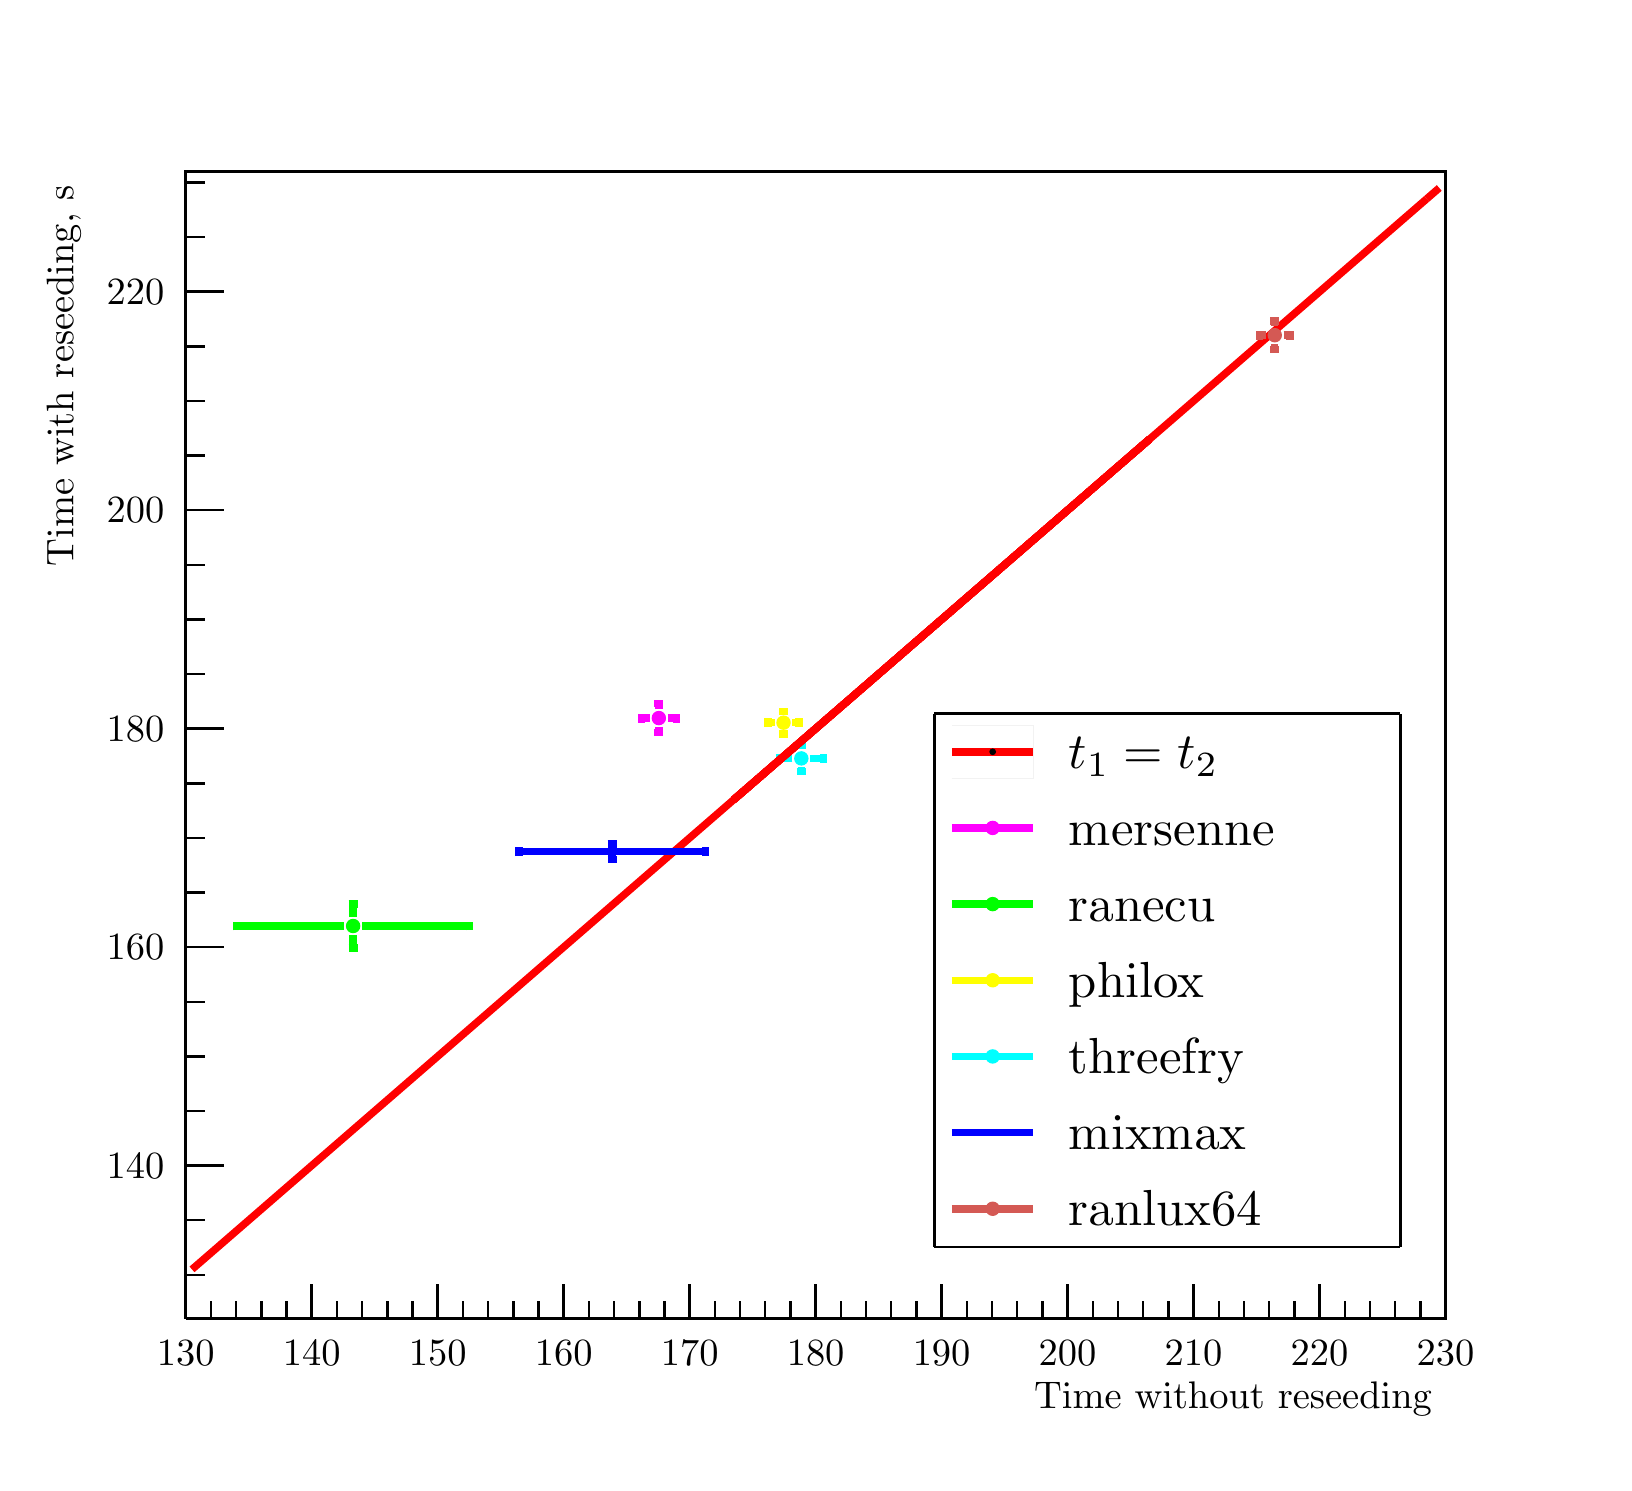
\begin{tikzpicture}
\pgfdeclareplotmark{cross} {
\pgfpathmoveto{\pgfpoint{-0.3\pgfplotmarksize}{\pgfplotmarksize}}
\pgfpathlineto{\pgfpoint{+0.3\pgfplotmarksize}{\pgfplotmarksize}}
\pgfpathlineto{\pgfpoint{+0.3\pgfplotmarksize}{0.3\pgfplotmarksize}}
\pgfpathlineto{\pgfpoint{+1\pgfplotmarksize}{0.3\pgfplotmarksize}}
\pgfpathlineto{\pgfpoint{+1\pgfplotmarksize}{-0.3\pgfplotmarksize}}
\pgfpathlineto{\pgfpoint{+0.3\pgfplotmarksize}{-0.3\pgfplotmarksize}}
\pgfpathlineto{\pgfpoint{+0.3\pgfplotmarksize}{-1.\pgfplotmarksize}}
\pgfpathlineto{\pgfpoint{-0.3\pgfplotmarksize}{-1.\pgfplotmarksize}}
\pgfpathlineto{\pgfpoint{-0.3\pgfplotmarksize}{-0.3\pgfplotmarksize}}
\pgfpathlineto{\pgfpoint{-1.\pgfplotmarksize}{-0.3\pgfplotmarksize}}
\pgfpathlineto{\pgfpoint{-1.\pgfplotmarksize}{0.3\pgfplotmarksize}}
\pgfpathlineto{\pgfpoint{-0.3\pgfplotmarksize}{0.3\pgfplotmarksize}}
\pgfpathclose
\pgfusepathqstroke
}
\pgfdeclareplotmark{cross*} {
\pgfpathmoveto{\pgfpoint{-0.3\pgfplotmarksize}{\pgfplotmarksize}}
\pgfpathlineto{\pgfpoint{+0.3\pgfplotmarksize}{\pgfplotmarksize}}
\pgfpathlineto{\pgfpoint{+0.3\pgfplotmarksize}{0.3\pgfplotmarksize}}
\pgfpathlineto{\pgfpoint{+1\pgfplotmarksize}{0.3\pgfplotmarksize}}
\pgfpathlineto{\pgfpoint{+1\pgfplotmarksize}{-0.3\pgfplotmarksize}}
\pgfpathlineto{\pgfpoint{+0.3\pgfplotmarksize}{-0.3\pgfplotmarksize}}
\pgfpathlineto{\pgfpoint{+0.3\pgfplotmarksize}{-1.\pgfplotmarksize}}
\pgfpathlineto{\pgfpoint{-0.3\pgfplotmarksize}{-1.\pgfplotmarksize}}
\pgfpathlineto{\pgfpoint{-0.3\pgfplotmarksize}{-0.3\pgfplotmarksize}}
\pgfpathlineto{\pgfpoint{-1.\pgfplotmarksize}{-0.3\pgfplotmarksize}}
\pgfpathlineto{\pgfpoint{-1.\pgfplotmarksize}{0.3\pgfplotmarksize}}
\pgfpathlineto{\pgfpoint{-0.3\pgfplotmarksize}{0.3\pgfplotmarksize}}
\pgfpathclose
\pgfusepathqfillstroke
}
\pgfdeclareplotmark{newstar} {
\pgfpathmoveto{\pgfqpoint{0pt}{\pgfplotmarksize}}
\pgfpathlineto{\pgfqpointpolar{44}{0.5\pgfplotmarksize}}
\pgfpathlineto{\pgfqpointpolar{18}{\pgfplotmarksize}}
\pgfpathlineto{\pgfqpointpolar{-20}{0.5\pgfplotmarksize}}
\pgfpathlineto{\pgfqpointpolar{-54}{\pgfplotmarksize}}
\pgfpathlineto{\pgfqpointpolar{-90}{0.5\pgfplotmarksize}}
\pgfpathlineto{\pgfqpointpolar{234}{\pgfplotmarksize}}
\pgfpathlineto{\pgfqpointpolar{198}{0.5\pgfplotmarksize}}
\pgfpathlineto{\pgfqpointpolar{162}{\pgfplotmarksize}}
\pgfpathlineto{\pgfqpointpolar{134}{0.5\pgfplotmarksize}}
\pgfpathclose
\pgfusepathqstroke
}
\pgfdeclareplotmark{newstar*} {
\pgfpathmoveto{\pgfqpoint{0pt}{\pgfplotmarksize}}
\pgfpathlineto{\pgfqpointpolar{44}{0.5\pgfplotmarksize}}
\pgfpathlineto{\pgfqpointpolar{18}{\pgfplotmarksize}}
\pgfpathlineto{\pgfqpointpolar{-20}{0.5\pgfplotmarksize}}
\pgfpathlineto{\pgfqpointpolar{-54}{\pgfplotmarksize}}
\pgfpathlineto{\pgfqpointpolar{-90}{0.5\pgfplotmarksize}}
\pgfpathlineto{\pgfqpointpolar{234}{\pgfplotmarksize}}
\pgfpathlineto{\pgfqpointpolar{198}{0.5\pgfplotmarksize}}
\pgfpathlineto{\pgfqpointpolar{162}{\pgfplotmarksize}}
\pgfpathlineto{\pgfqpointpolar{134}{0.5\pgfplotmarksize}}
\pgfpathclose
\pgfusepathqfillstroke
}
\definecolor{c}{rgb}{1,1,1};
\draw [color=c, fill=c] (0,0) rectangle (20,18.2077);
\draw [color=c, fill=c] (2,1.82077) rectangle (18,16.3869);
\definecolor{c}{rgb}{0,0,0};
\draw [c,line width=0.9] (2,1.82077) -- (2,16.3869) -- (18,16.3869) -- (18,1.82077) -- (2,1.82077);
\definecolor{c}{rgb}{1,1,1};
\draw [color=c, fill=c] (2,1.82077) rectangle (18,16.3869);
\definecolor{c}{rgb}{0,0,0};
\draw [c,line width=0.9] (2,1.82077) -- (2,16.3869) -- (18,16.3869) -- (18,1.82077) -- (2,1.82077);
\definecolor{c}{rgb}{1,0,0};
\draw [c,line width=2.7] (2.08,2.44503) -- (2.24,2.58376) -- (2.4,2.72248) -- (2.56,2.86121) -- (2.72,2.99993) -- (2.88,3.13866) -- (3.04,3.27738) -- (3.2,3.41611) -- (3.36,3.55483) -- (3.52,3.69356) -- (3.68,3.83228) -- (3.84,3.97101) -- (4,4.10973)
 -- (4.16,4.24846) -- (4.32,4.38718) -- (4.48,4.52591) -- (4.64,4.66463) -- (4.8,4.80336) -- (4.96,4.94209) -- (5.12,5.08081) -- (5.28,5.21954) -- (5.44,5.35826) -- (5.6,5.49699) -- (5.76,5.63571) -- (5.92,5.77444) -- (6.08,5.91316) -- (6.24,6.05189)
 -- (6.4,6.19061) -- (6.56,6.32934) -- (6.72,6.46806) -- (6.88,6.60679) -- (7.04,6.74551) -- (7.2,6.88424) -- (7.36,7.02296) -- (7.52,7.16169) -- (7.68,7.30041) -- (7.84,7.43914) -- (8,7.57786) -- (8.16,7.71659) -- (8.32,7.85531) -- (8.48,7.99404) --
 (8.64,8.13276) -- (8.8,8.27149) -- (8.96,8.41021) -- (9.12,8.54894) -- (9.28,8.68766) -- (9.44,8.82639) -- (9.6,8.96512) -- (9.76,9.10384) -- (9.92,9.24257);
\draw [c,line width=2.7] (9.92,9.24257) -- (10.08,9.38129) -- (10.24,9.52002) -- (10.4,9.65874) -- (10.56,9.79747) -- (10.72,9.93619) -- (10.88,10.0749) -- (11.04,10.2136) -- (11.2,10.3524) -- (11.36,10.4911) -- (11.52,10.6298) -- (11.68,10.7685) --
 (11.84,10.9073) -- (12,11.046) -- (12.16,11.1847) -- (12.32,11.3234) -- (12.48,11.4622) -- (12.64,11.6009) -- (12.8,11.7396) -- (12.96,11.8783) -- (13.12,12.0171) -- (13.28,12.1558) -- (13.44,12.2945) -- (13.6,12.4332) -- (13.76,12.572) --
 (13.92,12.7107) -- (14.08,12.8494) -- (14.24,12.9881) -- (14.4,13.1269) -- (14.56,13.2656) -- (14.72,13.4043) -- (14.88,13.543) -- (15.04,13.6818) -- (15.2,13.8205) -- (15.36,13.9592) -- (15.52,14.0979) -- (15.68,14.2367) -- (15.84,14.3754) --
 (16,14.5141) -- (16.16,14.6528) -- (16.32,14.7916) -- (16.48,14.9303) -- (16.64,15.069) -- (16.8,15.2077) -- (16.96,15.3465) -- (17.12,15.4852) -- (17.28,15.6239) -- (17.44,15.7627) -- (17.6,15.9014) -- (17.76,16.0401);
\draw [c,line width=2.7] (17.76,16.0401) -- (17.92,16.1788);
\definecolor{c}{rgb}{0,0,0};
\draw [c,line width=0.9] (2,1.82077) -- (18,1.82077);
\draw [c,line width=0.9] (2,2.25775) -- (2,1.82077);
\draw [c,line width=0.9] (2.32,2.03926) -- (2.32,1.82077);
\draw [c,line width=0.9] (2.64,2.03926) -- (2.64,1.82077);
\draw [c,line width=0.9] (2.96,2.03926) -- (2.96,1.82077);
\draw [c,line width=0.9] (3.28,2.03926) -- (3.28,1.82077);
\draw [c,line width=0.9] (3.6,2.25775) -- (3.6,1.82077);
\draw [c,line width=0.9] (3.92,2.03926) -- (3.92,1.82077);
\draw [c,line width=0.9] (4.24,2.03926) -- (4.24,1.82077);
\draw [c,line width=0.9] (4.56,2.03926) -- (4.56,1.82077);
\draw [c,line width=0.9] (4.88,2.03926) -- (4.88,1.82077);
\draw [c,line width=0.9] (5.2,2.25775) -- (5.2,1.82077);
\draw [c,line width=0.9] (5.52,2.03926) -- (5.52,1.82077);
\draw [c,line width=0.9] (5.84,2.03926) -- (5.84,1.82077);
\draw [c,line width=0.9] (6.16,2.03926) -- (6.16,1.82077);
\draw [c,line width=0.9] (6.48,2.03926) -- (6.48,1.82077);
\draw [c,line width=0.9] (6.8,2.25775) -- (6.8,1.82077);
\draw [c,line width=0.9] (7.12,2.03926) -- (7.12,1.82077);
\draw [c,line width=0.9] (7.44,2.03926) -- (7.44,1.82077);
\draw [c,line width=0.9] (7.76,2.03926) -- (7.76,1.82077);
\draw [c,line width=0.9] (8.08,2.03926) -- (8.08,1.82077);
\draw [c,line width=0.9] (8.4,2.25775) -- (8.4,1.82077);
\draw [c,line width=0.9] (8.72,2.03926) -- (8.72,1.82077);
\draw [c,line width=0.9] (9.04,2.03926) -- (9.04,1.82077);
\draw [c,line width=0.9] (9.36,2.03926) -- (9.36,1.82077);
\draw [c,line width=0.9] (9.68,2.03926) -- (9.68,1.82077);
\draw [c,line width=0.9] (10,2.25775) -- (10,1.82077);
\draw [c,line width=0.9] (10.32,2.03926) -- (10.32,1.82077);
\draw [c,line width=0.9] (10.64,2.03926) -- (10.64,1.82077);
\draw [c,line width=0.9] (10.96,2.03926) -- (10.96,1.82077);
\draw [c,line width=0.9] (11.28,2.03926) -- (11.28,1.82077);
\draw [c,line width=0.9] (11.6,2.25775) -- (11.6,1.82077);
\draw [c,line width=0.9] (11.92,2.03926) -- (11.92,1.82077);
\draw [c,line width=0.9] (12.24,2.03926) -- (12.24,1.82077);
\draw [c,line width=0.9] (12.56,2.03926) -- (12.56,1.82077);
\draw [c,line width=0.9] (12.88,2.03926) -- (12.88,1.82077);
\draw [c,line width=0.9] (13.2,2.25775) -- (13.2,1.82077);
\draw [c,line width=0.9] (13.52,2.03926) -- (13.52,1.82077);
\draw [c,line width=0.9] (13.84,2.03926) -- (13.84,1.82077);
\draw [c,line width=0.9] (14.16,2.03926) -- (14.16,1.82077);
\draw [c,line width=0.9] (14.48,2.03926) -- (14.48,1.82077);
\draw [c,line width=0.9] (14.8,2.25775) -- (14.8,1.82077);
\draw [c,line width=0.9] (15.12,2.03926) -- (15.12,1.82077);
\draw [c,line width=0.9] (15.44,2.03926) -- (15.44,1.82077);
\draw [c,line width=0.9] (15.76,2.03926) -- (15.76,1.82077);
\draw [c,line width=0.9] (16.08,2.03926) -- (16.08,1.82077);
\draw [c,line width=0.9] (16.4,2.25775) -- (16.4,1.82077);
\draw [c,line width=0.9] (16.72,2.03926) -- (16.72,1.82077);
\draw [c,line width=0.9] (17.04,2.03926) -- (17.04,1.82077);
\draw [c,line width=0.9] (17.36,2.03926) -- (17.36,1.82077);
\draw [c,line width=0.9] (17.68,2.03926) -- (17.68,1.82077);
\draw [c,line width=0.9] (18,2.25775) -- (18,1.82077);
\draw [anchor=base] (2,1.21991) node[scale=1.39008, color=c, rotate=0]{130};
\draw [anchor=base] (3.6,1.21991) node[scale=1.39008, color=c, rotate=0]{140};
\draw [anchor=base] (5.2,1.21991) node[scale=1.39008, color=c, rotate=0]{150};
\draw [anchor=base] (6.8,1.21991) node[scale=1.39008, color=c, rotate=0]{160};
\draw [anchor=base] (8.4,1.21991) node[scale=1.39008, color=c, rotate=0]{170};
\draw [anchor=base] (10,1.21991) node[scale=1.39008, color=c, rotate=0]{180};
\draw [anchor=base] (11.6,1.21991) node[scale=1.39008, color=c, rotate=0]{190};
\draw [anchor=base] (13.2,1.21991) node[scale=1.39008, color=c, rotate=0]{200};
\draw [anchor=base] (14.8,1.21991) node[scale=1.39008, color=c, rotate=0]{210};
\draw [anchor=base] (16.4,1.21991) node[scale=1.39008, color=c, rotate=0]{220};
\draw [anchor=base] (18,1.21991) node[scale=1.39008, color=c, rotate=0]{230};
\draw [anchor= east] (18,0.801138) node[scale=1.39008, color=c, rotate=0]{Time without reseeding};
\draw [c,line width=0.9] (2,1.82077) -- (2,16.3869);
\draw [c,line width=0.9] (2.48,3.76292) -- (2,3.76292);
\draw [c,line width=0.9] (2.24,4.45655) -- (2,4.45655);
\draw [c,line width=0.9] (2.24,5.15017) -- (2,5.15017);
\draw [c,line width=0.9] (2.24,5.8438) -- (2,5.8438);
\draw [c,line width=0.9] (2.48,6.53742) -- (2,6.53742);
\draw [c,line width=0.9] (2.24,7.23105) -- (2,7.23105);
\draw [c,line width=0.9] (2.24,7.92468) -- (2,7.92468);
\draw [c,line width=0.9] (2.24,8.6183) -- (2,8.6183);
\draw [c,line width=0.9] (2.48,9.31193) -- (2,9.31193);
\draw [c,line width=0.9] (2.24,10.0056) -- (2,10.0056);
\draw [c,line width=0.9] (2.24,10.6992) -- (2,10.6992);
\draw [c,line width=0.9] (2.24,11.3928) -- (2,11.3928);
\draw [c,line width=0.9] (2.48,12.0864) -- (2,12.0864);
\draw [c,line width=0.9] (2.24,12.7801) -- (2,12.7801);
\draw [c,line width=0.9] (2.24,13.4737) -- (2,13.4737);
\draw [c,line width=0.9] (2.24,14.1673) -- (2,14.1673);
\draw [c,line width=0.9] (2.48,14.8609) -- (2,14.8609);
\draw [c,line width=0.9] (2.48,3.76292) -- (2,3.76292);
\draw [c,line width=0.9] (2.24,3.06929) -- (2,3.06929);
\draw [c,line width=0.9] (2.24,2.37567) -- (2,2.37567);
\draw [c,line width=0.9] (2.48,14.8609) -- (2,14.8609);
\draw [c,line width=0.9] (2.24,15.5546) -- (2,15.5546);
\draw [c,line width=0.9] (2.24,16.2482) -- (2,16.2482);
\draw [anchor= east] (1.9,3.76292) node[scale=1.39008, color=c, rotate=0]{140};
\draw [anchor= east] (1.9,6.53742) node[scale=1.39008, color=c, rotate=0]{160};
\draw [anchor= east] (1.9,9.31193) node[scale=1.39008, color=c, rotate=0]{180};
\draw [anchor= east] (1.9,12.0864) node[scale=1.39008, color=c, rotate=0]{200};
\draw [anchor= east] (1.9,14.8609) node[scale=1.39008, color=c, rotate=0]{220};
\draw [anchor= east] (0.452347,16.3869) node[scale=1.39008, color=c, rotate=90]{Time with reseeding, s};
\definecolor{c}{rgb}{1,0,1};
\draw [c,line width=2.7] (7.895,9.44658) -- (7.7853,9.44658);
\draw [c,line width=2.7] (7.7853,9.38968) -- (7.7853,9.50348);
\draw [c,line width=2.7] (8.1226,9.44658) -- (8.2323,9.44658);
\draw [c,line width=2.7] (8.2323,9.38968) -- (8.2323,9.50348);
\draw [c,line width=2.7] (8.0088,9.56038) -- (8.0088,9.63112);
\draw [c,line width=2.7] (7.9519,9.63112) -- (8.0657,9.63112);
\draw [c,line width=2.7] (8.0088,9.33278) -- (8.0088,9.26204);
\draw [c,line width=2.7] (7.9519,9.26204) -- (8.0657,9.26204);
\foreach \P in {(8.0088,9.44658)}{\draw[mark options={color=c,fill=c},mark size=2.402402pt,mark=*] plot coordinates {\P};}
\definecolor{c}{rgb}{0,1,0};
\draw [c,line width=2.7] (4.0123,6.80586) -- (2.64491,6.80586);
\draw [c,line width=2.7] (2.64491,6.74896) -- (2.64491,6.86276);
\draw [c,line width=2.7] (4.2399,6.80586) -- (5.60729,6.80586);
\draw [c,line width=2.7] (5.60729,6.74896) -- (5.60729,6.86276);
\draw [c,line width=2.7] (4.1261,6.91966) -- (4.1261,7.08758);
\draw [c,line width=2.7] (4.0692,7.08758) -- (4.183,7.08758);
\draw [c,line width=2.7] (4.1261,6.69206) -- (4.1261,6.52414);
\draw [c,line width=2.7] (4.0692,6.52414) -- (4.183,6.52414);
\foreach \P in {(4.1261,6.80586)}{\draw[mark options={color=c,fill=c},mark size=2.402402pt,mark=*] plot coordinates {\P};}
\definecolor{c}{rgb}{1,1,0};
\draw [c,line width=2.7] (9.4785,9.38823) -- (9.3968,9.38823);
\draw [c,line width=2.7] (9.3968,9.33133) -- (9.3968,9.44513);
\draw [c,line width=2.7] (9.7061,9.38823) -- (9.7878,9.38823);
\draw [c,line width=2.7] (9.7878,9.33133) -- (9.7878,9.44513);
\draw [c,line width=2.7] (9.5923,9.50203) -- (9.5923,9.53051);
\draw [c,line width=2.7] (9.5354,9.53051) -- (9.6492,9.53051);
\draw [c,line width=2.7] (9.5923,9.27443) -- (9.5923,9.24595);
\draw [c,line width=2.7] (9.5354,9.24595) -- (9.6492,9.24595);
\foreach \P in {(9.5923,9.38823)}{\draw[mark options={color=c,fill=c},mark size=2.402402pt,mark=*] plot coordinates {\P};}
\definecolor{c}{rgb}{0,1,1};
\draw [c,line width=2.7] (9.7045,8.93434) -- (9.53897,8.93434);
\draw [c,line width=2.7] (9.53897,8.87744) -- (9.53897,8.99123);
\draw [c,line width=2.7] (9.9321,8.93434) -- (10.0976,8.93434);
\draw [c,line width=2.7] (10.0976,8.87744) -- (10.0976,8.99123);
\draw [c,line width=2.7] (9.8183,9.04813) -- (9.8183,9.09913);
\draw [c,line width=2.7] (9.7614,9.09913) -- (9.8752,9.09913);
\draw [c,line width=2.7] (9.8183,8.82054) -- (9.8183,8.76955);
\draw [c,line width=2.7] (9.7614,8.76955) -- (9.8752,8.76955);
\foreach \P in {(9.8183,8.93434)}{\draw[mark options={color=c,fill=c},mark size=2.402402pt,mark=*] plot coordinates {\P};}
\definecolor{c}{rgb}{0,0,1};
\draw [c,line width=2.7] (7.4154,7.74919) -- (6.23044,7.74919);
\draw [c,line width=2.7] (6.23044,7.69229) -- (6.23044,7.80609);
\draw [c,line width=2.7] (7.4154,7.74919) -- (8.60036,7.74919);
\draw [c,line width=2.7] (8.60036,7.69229) -- (8.60036,7.80609);
\draw [c,line width=2.7] (7.4154,7.74919) -- (7.4154,7.84836);
\draw [c,line width=2.7] (7.3585,7.84836) -- (7.4723,7.84836);
\draw [c,line width=2.7] (7.4154,7.74919) -- (7.4154,7.65002);
\draw [c,line width=2.7] (7.3585,7.65002) -- (7.4723,7.65002);
\foreach \P in {(7.4154,7.74919)}{\draw[mark options={color=c,fill=c},mark size=2.402402pt,mark=] plot coordinates {\P};}
\definecolor{c}{rgb}{0.83,0.35,0.33};
\draw [c,line width=2.7] (15.717,14.3089) -- (15.6367,14.3089);
\draw [c,line width=2.7] (15.6367,14.252) -- (15.6367,14.3658);
\draw [c,line width=2.7] (15.9446,14.3089) -- (16.0249,14.3089);
\draw [c,line width=2.7] (16.0249,14.252) -- (16.0249,14.3658);
\draw [c,line width=2.7] (15.8308,14.4227) -- (15.8308,14.4883);
\draw [c,line width=2.7] (15.7739,14.4883) -- (15.8877,14.4883);
\draw [c,line width=2.7] (15.8308,14.1951) -- (15.8308,14.1295);
\draw [c,line width=2.7] (15.7739,14.1295) -- (15.8877,14.1295);
\foreach \P in {(15.8308,14.3089)}{\draw[mark options={color=c,fill=c},mark size=2.402402pt,mark=*] plot coordinates {\P};}
\definecolor{c}{rgb}{1,1,1};
\draw [color=c, fill=c] (11.5089,2.73115) rectangle (17.426,9.50213);
\definecolor{c}{rgb}{0,0,0};
\draw [c,line width=0.9] (11.5089,2.73115) -- (17.426,2.73115);
\draw [c,line width=0.9] (17.426,2.73115) -- (17.426,9.50213);
\draw [c,line width=0.9] (17.426,9.50213) -- (11.5089,9.50213);
\draw [c,line width=0.9] (11.5089,9.50213) -- (11.5089,2.73115);
\draw [anchor=base west] (12.9882,8.80085) node[scale=1.83238, color=c, rotate=0]{$t_{1} = t_{2}$};
\definecolor{c}{rgb}{0.95,0.95,0.95};
\draw [c] (11.7308,8.67994) -- (12.7663,8.67994) -- (12.7663,9.35704) -- (11.7308,9.35704);
\definecolor{c}{rgb}{1,0,0};
\draw [c,line width=2.7] (11.7308,9.01849) -- (12.7663,9.01849);
\definecolor{c}{rgb}{0,0,0};
\foreach \P in {(12.2485,9.01849)}{\draw[mark options={color=c,fill=c},mark size=2.402402pt,mark=*,mark size=1pt] plot coordinates {\P};}
\draw [anchor=base west] (12.9882,7.83357) node[scale=1.83238, color=c, rotate=0]{mersenne};
\definecolor{c}{rgb}{1,1,1};
\draw [c] (11.7308,7.71266) -- (12.7663,7.71266) -- (12.7663,8.38976) -- (11.7308,8.38976);
\definecolor{c}{rgb}{1,0,1};
\draw [c,line width=2.7] (11.7308,8.05121) -- (12.7663,8.05121);
\foreach \P in {(12.2485,8.05121)}{\draw[mark options={color=c,fill=c},mark size=2.402402pt,mark=*] plot coordinates {\P};}
\definecolor{c}{rgb}{0,0,0};
\draw [anchor=base west] (12.9882,6.86629) node[scale=1.83238, color=c, rotate=0]{ranecu};
\definecolor{c}{rgb}{1,1,1};
\draw [c] (11.7308,6.74538) -- (12.7663,6.74538) -- (12.7663,7.42248) -- (11.7308,7.42248);
\definecolor{c}{rgb}{0,1,0};
\draw [c,line width=2.7] (11.7308,7.08393) -- (12.7663,7.08393);
\foreach \P in {(12.2485,7.08393)}{\draw[mark options={color=c,fill=c},mark size=2.402402pt,mark=*] plot coordinates {\P};}
\definecolor{c}{rgb}{0,0,0};
\draw [anchor=base west] (12.9882,5.899) node[scale=1.83238, color=c, rotate=0]{philox};
\definecolor{c}{rgb}{1,1,1};
\draw [c] (11.7308,5.77809) -- (12.7663,5.77809) -- (12.7663,6.45519) -- (11.7308,6.45519);
\definecolor{c}{rgb}{1,1,0};
\draw [c,line width=2.7] (11.7308,6.11664) -- (12.7663,6.11664);
\foreach \P in {(12.2485,6.11664)}{\draw[mark options={color=c,fill=c},mark size=2.402402pt,mark=*] plot coordinates {\P};}
\definecolor{c}{rgb}{0,0,0};
\draw [anchor=base west] (12.9882,4.93172) node[scale=1.83238, color=c, rotate=0]{threefry};
\definecolor{c}{rgb}{1,1,1};
\draw [c] (11.7308,4.81081) -- (12.7663,4.81081) -- (12.7663,5.48791) -- (11.7308,5.48791);
\definecolor{c}{rgb}{0,1,1};
\draw [c,line width=2.7] (11.7308,5.14936) -- (12.7663,5.14936);
\foreach \P in {(12.2485,5.14936)}{\draw[mark options={color=c,fill=c},mark size=2.402402pt,mark=*] plot coordinates {\P};}
\definecolor{c}{rgb}{0,0,0};
\draw [anchor=base west] (12.9882,3.96444) node[scale=1.83238, color=c, rotate=0]{mixmax};
\definecolor{c}{rgb}{1,1,1};
\draw [c] (11.7308,3.84353) -- (12.7663,3.84353) -- (12.7663,4.52063) -- (11.7308,4.52063);
\definecolor{c}{rgb}{0,0,1};
\draw [c,line width=2.7] (11.7308,4.18208) -- (12.7663,4.18208);
\foreach \P in {(12.2485,4.18208)}{\draw[mark options={color=c,fill=c},mark size=2.402402pt,mark=] plot coordinates {\P};}
\definecolor{c}{rgb}{0,0,0};
\draw [anchor=base west] (12.9882,2.99716) node[scale=1.83238, color=c, rotate=0]{ranlux64};
\definecolor{c}{rgb}{1,1,1};
\draw [c] (11.7308,2.87624) -- (12.7663,2.87624) -- (12.7663,3.55334) -- (11.7308,3.55334);
\definecolor{c}{rgb}{0.83,0.35,0.33};
\draw [c,line width=2.7] (11.7308,3.21479) -- (12.7663,3.21479);
\foreach \P in {(12.2485,3.21479)}{\draw[mark options={color=c,fill=c},mark size=2.402402pt,mark=*] plot coordinates {\P};}
\definecolor{c}{rgb}{1,0,0};
\draw [c,line width=2.7] (8.96,8.41021) -- (9.01333,8.45646) -- (9.06667,8.5027) -- (9.12,8.54894) -- (9.17333,8.59518) -- (9.22667,8.64142) -- (9.28,8.68766) -- (9.33333,8.73391) -- (9.38667,8.78015) -- (9.44,8.82639) -- (9.49333,8.87263) --
 (9.54667,8.91887) -- (9.6,8.96512) -- (9.65333,9.01136) -- (9.70667,9.0576) -- (9.76,9.10384) -- (9.81333,9.15008) -- (9.86667,9.19632) -- (9.92,9.24257) -- (9.97333,9.28881) -- (10.0267,9.33505) -- (10.08,9.38129) -- (10.1333,9.42753) --
 (10.1867,9.47377) -- (10.24,9.52002) -- (10.2933,9.56626) -- (10.3467,9.6125) -- (10.4,9.65874) -- (10.4533,9.70498) -- (10.5067,9.75123) -- (10.56,9.79747) -- (10.6133,9.84371) -- (10.6667,9.88995) -- (10.72,9.93619) -- (10.7733,9.98243) --
 (10.8267,10.0287) -- (10.88,10.0749) -- (10.9333,10.1212) -- (10.9867,10.1674) -- (11.04,10.2136) -- (11.0933,10.2599) -- (11.1467,10.3061) -- (11.2,10.3524) -- (11.2533,10.3986) -- (11.3067,10.4449) -- (11.36,10.4911) -- (11.4133,10.5373) --
 (11.4667,10.5836) -- (11.52,10.6298) -- (11.5733,10.6761);
\draw [c,line width=2.7] (11.5733,10.6761) -- (11.6267,10.7223) -- (11.68,10.7685) -- (11.7333,10.8148) -- (11.7867,10.861) -- (11.84,10.9073) -- (11.8933,10.9535) -- (11.9467,10.9998) -- (12,11.046) -- (12.0533,11.0922) -- (12.1067,11.1385) --
 (12.16,11.1847) -- (12.2133,11.231) -- (12.2667,11.2772) -- (12.32,11.3234) -- (12.3733,11.3697) -- (12.4267,11.4159) -- (12.48,11.4622) -- (12.5333,11.5084) -- (12.5867,11.5547) -- (12.64,11.6009) -- (12.6933,11.6471) -- (12.7467,11.6934) --
 (12.8,11.7396) -- (12.8533,11.7859) -- (12.9067,11.8321) -- (12.96,11.8783) -- (13.0133,11.9246) -- (13.0667,11.9708) -- (13.12,12.0171) -- (13.1733,12.0633) -- (13.2267,12.1096) -- (13.28,12.1558) -- (13.3333,12.202) -- (13.3867,12.2483) --
 (13.44,12.2945) -- (13.4933,12.3408) -- (13.5467,12.387) -- (13.6,12.4332) -- (13.6533,12.4795) -- (13.7067,12.5257) -- (13.76,12.572) -- (13.8133,12.6182) -- (13.8667,12.6645) -- (13.92,12.7107) -- (13.9733,12.7569) -- (14.0267,12.8032) --
 (14.08,12.8494) -- (14.1333,12.8957) -- (14.1867,12.9419);
\draw [c,line width=2.7] (14.1867,12.9419) -- (14.24,12.9881);
\draw [c,line width=2.7] (8.96,8.41021) -- (9.01333,8.45646) -- (9.06667,8.5027) -- (9.12,8.54894) -- (9.17333,8.59518) -- (9.22667,8.64142) -- (9.28,8.68766) -- (9.33333,8.73391) -- (9.38667,8.78015) -- (9.44,8.82639) -- (9.49333,8.87263) --
 (9.54667,8.91887) -- (9.6,8.96512) -- (9.65333,9.01136) -- (9.70667,9.0576) -- (9.76,9.10384) -- (9.81333,9.15008) -- (9.86667,9.19632) -- (9.92,9.24257) -- (9.97333,9.28881) -- (10.0267,9.33505) -- (10.08,9.38129) -- (10.1333,9.42753) --
 (10.1867,9.47377) -- (10.24,9.52002) -- (10.2933,9.56626) -- (10.3467,9.6125) -- (10.4,9.65874) -- (10.4533,9.70498) -- (10.5067,9.75123) -- (10.56,9.79747) -- (10.6133,9.84371) -- (10.6667,9.88995) -- (10.72,9.93619) -- (10.7733,9.98243) --
 (10.8267,10.0287) -- (10.88,10.0749) -- (10.9333,10.1212) -- (10.9867,10.1674) -- (11.04,10.2136) -- (11.0933,10.2599) -- (11.1467,10.3061) -- (11.2,10.3524) -- (11.2533,10.3986) -- (11.3067,10.4449) -- (11.36,10.4911) -- (11.4133,10.5373) --
 (11.4667,10.5836) -- (11.52,10.6298) -- (11.5733,10.6761);
\draw [c,line width=2.7] (11.5733,10.6761) -- (11.6267,10.7223) -- (11.68,10.7685) -- (11.7333,10.8148) -- (11.7867,10.861) -- (11.84,10.9073) -- (11.8933,10.9535) -- (11.9467,10.9998) -- (12,11.046) -- (12.0533,11.0922) -- (12.1067,11.1385) --
 (12.16,11.1847) -- (12.2133,11.231) -- (12.2667,11.2772) -- (12.32,11.3234) -- (12.3733,11.3697) -- (12.4267,11.4159) -- (12.48,11.4622) -- (12.5333,11.5084) -- (12.5867,11.5547) -- (12.64,11.6009) -- (12.6933,11.6471) -- (12.7467,11.6934) --
 (12.8,11.7396) -- (12.8533,11.7859) -- (12.9067,11.8321) -- (12.96,11.8783) -- (13.0133,11.9246) -- (13.0667,11.9708) -- (13.12,12.0171) -- (13.1733,12.0633) -- (13.2267,12.1096) -- (13.28,12.1558) -- (13.3333,12.202) -- (13.3867,12.2483) --
 (13.44,12.2945) -- (13.4933,12.3408) -- (13.5467,12.387) -- (13.6,12.4332) -- (13.6533,12.4795) -- (13.7067,12.5257) -- (13.76,12.572) -- (13.8133,12.6182) -- (13.8667,12.6645) -- (13.92,12.7107) -- (13.9733,12.7569) -- (14.0267,12.8032) --
 (14.08,12.8494) -- (14.1333,12.8957) -- (14.1867,12.9419);
\draw [c,line width=2.7] (14.1867,12.9419) -- (14.24,12.9881);
\draw [c,line width=2.7] (8.96,8.41021) -- (9.01333,8.45646) -- (9.06667,8.5027) -- (9.12,8.54894) -- (9.17333,8.59518) -- (9.22667,8.64142) -- (9.28,8.68766) -- (9.33333,8.73391) -- (9.38667,8.78015) -- (9.44,8.82639) -- (9.49333,8.87263) --
 (9.54667,8.91887) -- (9.6,8.96512) -- (9.65333,9.01136) -- (9.70667,9.0576) -- (9.76,9.10384) -- (9.81333,9.15008) -- (9.86667,9.19632) -- (9.92,9.24257) -- (9.97333,9.28881) -- (10.0267,9.33505) -- (10.08,9.38129) -- (10.1333,9.42753) --
 (10.1867,9.47377) -- (10.24,9.52002) -- (10.2933,9.56626) -- (10.3467,9.6125) -- (10.4,9.65874) -- (10.4533,9.70498) -- (10.5067,9.75123) -- (10.56,9.79747) -- (10.6133,9.84371) -- (10.6667,9.88995) -- (10.72,9.93619) -- (10.7733,9.98243) --
 (10.8267,10.0287) -- (10.88,10.0749) -- (10.9333,10.1212) -- (10.9867,10.1674) -- (11.04,10.2136) -- (11.0933,10.2599) -- (11.1467,10.3061) -- (11.2,10.3524) -- (11.2533,10.3986) -- (11.3067,10.4449) -- (11.36,10.4911) -- (11.4133,10.5373) --
 (11.4667,10.5836) -- (11.52,10.6298) -- (11.5733,10.6761);
\draw [c,line width=2.7] (11.5733,10.6761) -- (11.6267,10.7223) -- (11.68,10.7685) -- (11.7333,10.8148) -- (11.7867,10.861) -- (11.84,10.9073) -- (11.8933,10.9535) -- (11.9467,10.9998) -- (12,11.046) -- (12.0533,11.0922) -- (12.1067,11.1385) --
 (12.16,11.1847) -- (12.2133,11.231) -- (12.2667,11.2772) -- (12.32,11.3234) -- (12.3733,11.3697) -- (12.4267,11.4159) -- (12.48,11.4622) -- (12.5333,11.5084) -- (12.5867,11.5547) -- (12.64,11.6009) -- (12.6933,11.6471) -- (12.7467,11.6934) --
 (12.8,11.7396) -- (12.8533,11.7859) -- (12.9067,11.8321) -- (12.96,11.8783) -- (13.0133,11.9246) -- (13.0667,11.9708) -- (13.12,12.0171) -- (13.1733,12.0633) -- (13.2267,12.1096) -- (13.28,12.1558) -- (13.3333,12.202) -- (13.3867,12.2483) --
 (13.44,12.2945) -- (13.4933,12.3408) -- (13.5467,12.387) -- (13.6,12.4332) -- (13.6533,12.4795) -- (13.7067,12.5257) -- (13.76,12.572) -- (13.8133,12.6182) -- (13.8667,12.6645) -- (13.92,12.7107) -- (13.9733,12.7569) -- (14.0267,12.8032) --
 (14.08,12.8494) -- (14.1333,12.8957) -- (14.1867,12.9419);
\draw [c,line width=2.7] (14.1867,12.9419) -- (14.24,12.9881);
\draw [c,line width=2.7] (8.96,8.41021) -- (9.01333,8.45646) -- (9.06667,8.5027) -- (9.12,8.54894) -- (9.17333,8.59518) -- (9.22667,8.64142) -- (9.28,8.68766) -- (9.33333,8.73391) -- (9.38667,8.78015) -- (9.44,8.82639) -- (9.49333,8.87263) --
 (9.54667,8.91887) -- (9.6,8.96512) -- (9.65333,9.01136) -- (9.70667,9.0576) -- (9.76,9.10384) -- (9.81333,9.15008) -- (9.86667,9.19632) -- (9.92,9.24257) -- (9.97333,9.28881) -- (10.0267,9.33505) -- (10.08,9.38129) -- (10.1333,9.42753) --
 (10.1867,9.47377) -- (10.24,9.52002) -- (10.2933,9.56626) -- (10.3467,9.6125) -- (10.4,9.65874) -- (10.4533,9.70498) -- (10.5067,9.75123) -- (10.56,9.79747) -- (10.6133,9.84371) -- (10.6667,9.88995) -- (10.72,9.93619) -- (10.7733,9.98243) --
 (10.8267,10.0287) -- (10.88,10.0749) -- (10.9333,10.1212) -- (10.9867,10.1674) -- (11.04,10.2136) -- (11.0933,10.2599) -- (11.1467,10.3061) -- (11.2,10.3524) -- (11.2533,10.3986) -- (11.3067,10.4449) -- (11.36,10.4911) -- (11.4133,10.5373) --
 (11.4667,10.5836) -- (11.52,10.6298) -- (11.5733,10.6761);
\draw [c,line width=2.7] (11.5733,10.6761) -- (11.6267,10.7223) -- (11.68,10.7685) -- (11.7333,10.8148) -- (11.7867,10.861) -- (11.84,10.9073) -- (11.8933,10.9535) -- (11.9467,10.9998) -- (12,11.046) -- (12.0533,11.0922) -- (12.1067,11.1385) --
 (12.16,11.1847) -- (12.2133,11.231) -- (12.2667,11.2772) -- (12.32,11.3234) -- (12.3733,11.3697) -- (12.4267,11.4159) -- (12.48,11.4622) -- (12.5333,11.5084) -- (12.5867,11.5547) -- (12.64,11.6009) -- (12.6933,11.6471) -- (12.7467,11.6934) --
 (12.8,11.7396) -- (12.8533,11.7859) -- (12.9067,11.8321) -- (12.96,11.8783) -- (13.0133,11.9246) -- (13.0667,11.9708) -- (13.12,12.0171) -- (13.1733,12.0633) -- (13.2267,12.1096) -- (13.28,12.1558) -- (13.3333,12.202) -- (13.3867,12.2483) --
 (13.44,12.2945) -- (13.4933,12.3408) -- (13.5467,12.387) -- (13.6,12.4332) -- (13.6533,12.4795) -- (13.7067,12.5257) -- (13.76,12.572) -- (13.8133,12.6182) -- (13.8667,12.6645) -- (13.92,12.7107) -- (13.9733,12.7569) -- (14.0267,12.8032) --
 (14.08,12.8494) -- (14.1333,12.8957) -- (14.1867,12.9419);
\draw [c,line width=2.7] (14.1867,12.9419) -- (14.24,12.9881);
\draw [c,line width=2.7] (8.96,8.41021) -- (9.01333,8.45646) -- (9.06667,8.5027) -- (9.12,8.54894) -- (9.17333,8.59518) -- (9.22667,8.64142) -- (9.28,8.68766) -- (9.33333,8.73391) -- (9.38667,8.78015) -- (9.44,8.82639) -- (9.49333,8.87263) --
 (9.54667,8.91887) -- (9.6,8.96512) -- (9.65333,9.01136) -- (9.70667,9.0576) -- (9.76,9.10384) -- (9.81333,9.15008) -- (9.86667,9.19632) -- (9.92,9.24257) -- (9.97333,9.28881) -- (10.0267,9.33505) -- (10.08,9.38129) -- (10.1333,9.42753) --
 (10.1867,9.47377) -- (10.24,9.52002) -- (10.2933,9.56626) -- (10.3467,9.6125) -- (10.4,9.65874) -- (10.4533,9.70498) -- (10.5067,9.75123) -- (10.56,9.79747) -- (10.6133,9.84371) -- (10.6667,9.88995) -- (10.72,9.93619) -- (10.7733,9.98243) --
 (10.8267,10.0287) -- (10.88,10.0749) -- (10.9333,10.1212) -- (10.9867,10.1674) -- (11.04,10.2136) -- (11.0933,10.2599) -- (11.1467,10.3061) -- (11.2,10.3524) -- (11.2533,10.3986) -- (11.3067,10.4449) -- (11.36,10.4911) -- (11.4133,10.5373) --
 (11.4667,10.5836) -- (11.52,10.6298) -- (11.5733,10.6761);
\draw [c,line width=2.7] (11.5733,10.6761) -- (11.6267,10.7223) -- (11.68,10.7685) -- (11.7333,10.8148) -- (11.7867,10.861) -- (11.84,10.9073) -- (11.8933,10.9535) -- (11.9467,10.9998) -- (12,11.046) -- (12.0533,11.0922) -- (12.1067,11.1385) --
 (12.16,11.1847) -- (12.2133,11.231) -- (12.2667,11.2772) -- (12.32,11.3234) -- (12.3733,11.3697) -- (12.4267,11.4159) -- (12.48,11.4622) -- (12.5333,11.5084) -- (12.5867,11.5547) -- (12.64,11.6009) -- (12.6933,11.6471) -- (12.7467,11.6934) --
 (12.8,11.7396) -- (12.8533,11.7859) -- (12.9067,11.8321) -- (12.96,11.8783) -- (13.0133,11.9246) -- (13.0667,11.9708) -- (13.12,12.0171) -- (13.1733,12.0633) -- (13.2267,12.1096) -- (13.28,12.1558) -- (13.3333,12.202) -- (13.3867,12.2483) --
 (13.44,12.2945) -- (13.4933,12.3408) -- (13.5467,12.387) -- (13.6,12.4332) -- (13.6533,12.4795) -- (13.7067,12.5257) -- (13.76,12.572) -- (13.8133,12.6182) -- (13.8667,12.6645) -- (13.92,12.7107) -- (13.9733,12.7569) -- (14.0267,12.8032) --
 (14.08,12.8494) -- (14.1333,12.8957) -- (14.1867,12.9419);
\draw [c,line width=2.7] (14.1867,12.9419) -- (14.24,12.9881);
\draw [c,line width=2.7] (8.96,8.41021) -- (9.01333,8.45646) -- (9.06667,8.5027) -- (9.12,8.54894) -- (9.17333,8.59518) -- (9.22667,8.64142) -- (9.28,8.68766) -- (9.33333,8.73391) -- (9.38667,8.78015) -- (9.44,8.82639) -- (9.49333,8.87263) --
 (9.54667,8.91887) -- (9.6,8.96512) -- (9.65333,9.01136) -- (9.70667,9.0576) -- (9.76,9.10384) -- (9.81333,9.15008) -- (9.86667,9.19632) -- (9.92,9.24257) -- (9.97333,9.28881) -- (10.0267,9.33505) -- (10.08,9.38129) -- (10.1333,9.42753) --
 (10.1867,9.47377) -- (10.24,9.52002) -- (10.2933,9.56626) -- (10.3467,9.6125) -- (10.4,9.65874) -- (10.4533,9.70498) -- (10.5067,9.75123) -- (10.56,9.79747) -- (10.6133,9.84371) -- (10.6667,9.88995) -- (10.72,9.93619) -- (10.7733,9.98243) --
 (10.8267,10.0287) -- (10.88,10.0749) -- (10.9333,10.1212) -- (10.9867,10.1674) -- (11.04,10.2136) -- (11.0933,10.2599) -- (11.1467,10.3061) -- (11.2,10.3524) -- (11.2533,10.3986) -- (11.3067,10.4449) -- (11.36,10.4911) -- (11.4133,10.5373) --
 (11.4667,10.5836) -- (11.52,10.6298) -- (11.5733,10.6761);
\draw [c,line width=2.7] (11.5733,10.6761) -- (11.6267,10.7223) -- (11.68,10.7685) -- (11.7333,10.8148) -- (11.7867,10.861) -- (11.84,10.9073) -- (11.8933,10.9535) -- (11.9467,10.9998) -- (12,11.046) -- (12.0533,11.0922) -- (12.1067,11.1385) --
 (12.16,11.1847) -- (12.2133,11.231) -- (12.2667,11.2772) -- (12.32,11.3234) -- (12.3733,11.3697) -- (12.4267,11.4159) -- (12.48,11.4622) -- (12.5333,11.5084) -- (12.5867,11.5547) -- (12.64,11.6009) -- (12.6933,11.6471) -- (12.7467,11.6934) --
 (12.8,11.7396) -- (12.8533,11.7859) -- (12.9067,11.8321) -- (12.96,11.8783) -- (13.0133,11.9246) -- (13.0667,11.9708) -- (13.12,12.0171) -- (13.1733,12.0633) -- (13.2267,12.1096) -- (13.28,12.1558) -- (13.3333,12.202) -- (13.3867,12.2483) --
 (13.44,12.2945) -- (13.4933,12.3408) -- (13.5467,12.387) -- (13.6,12.4332) -- (13.6533,12.4795) -- (13.7067,12.5257) -- (13.76,12.572) -- (13.8133,12.6182) -- (13.8667,12.6645) -- (13.92,12.7107) -- (13.9733,12.7569) -- (14.0267,12.8032) --
 (14.08,12.8494) -- (14.1333,12.8957) -- (14.1867,12.9419);
\draw [c,line width=2.7] (14.1867,12.9419) -- (14.24,12.9881);
\end{tikzpicture}
}  
% %    \caption{Caption A}
%     \label{fig:A}
   \end{subfloat}
   \begin{subfloat}[][]
    \centering
    \scalebox{.33}{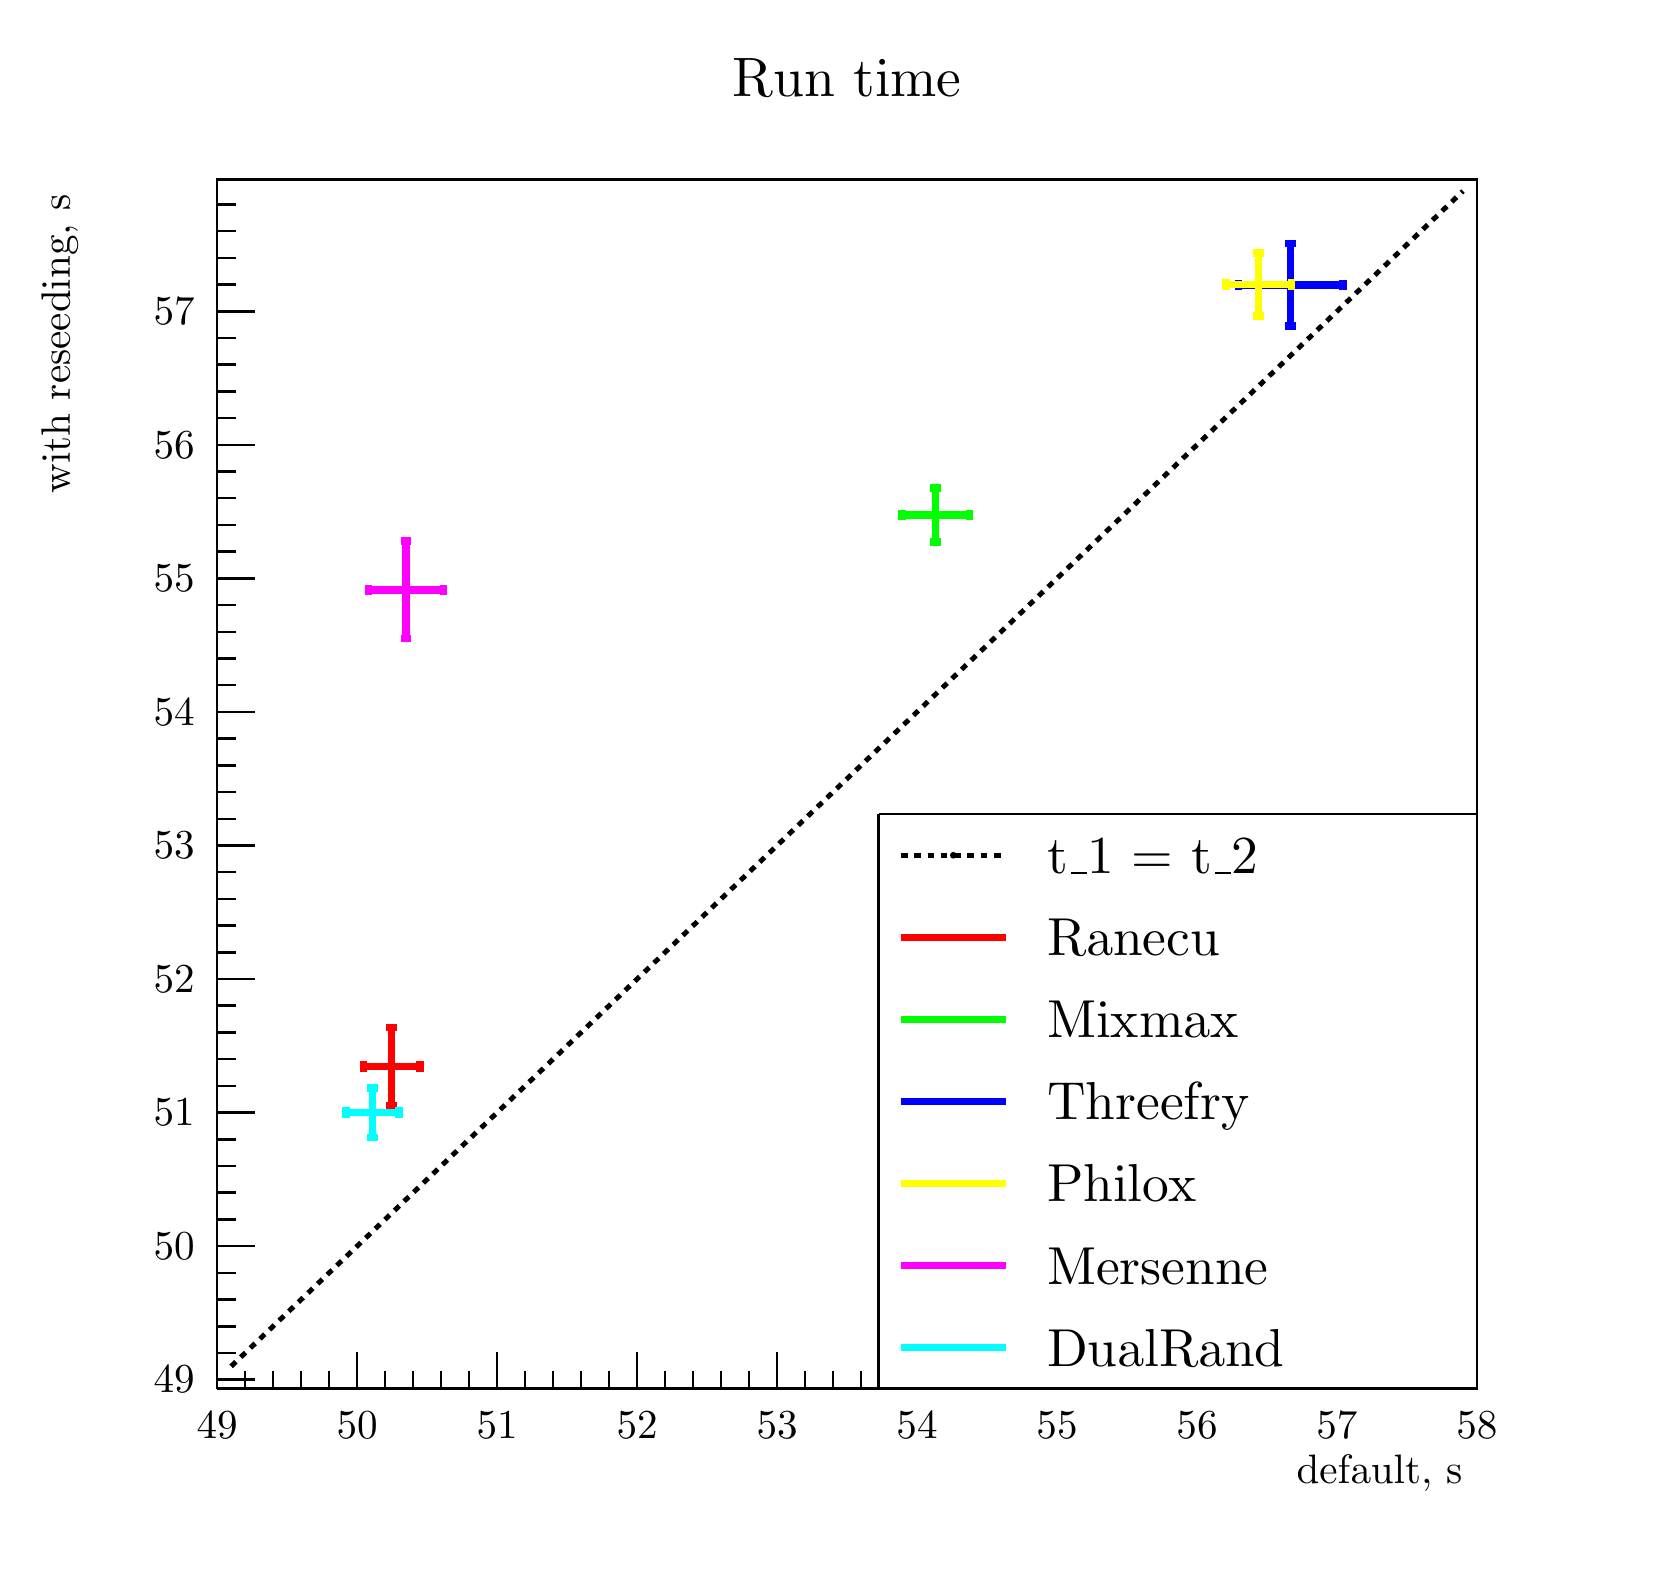
\begin{tikzpicture}
\pgfdeclareplotmark{cross} {
\pgfpathmoveto{\pgfpoint{-0.3\pgfplotmarksize}{\pgfplotmarksize}}
\pgfpathlineto{\pgfpoint{+0.3\pgfplotmarksize}{\pgfplotmarksize}}
\pgfpathlineto{\pgfpoint{+0.3\pgfplotmarksize}{0.3\pgfplotmarksize}}
\pgfpathlineto{\pgfpoint{+1\pgfplotmarksize}{0.3\pgfplotmarksize}}
\pgfpathlineto{\pgfpoint{+1\pgfplotmarksize}{-0.3\pgfplotmarksize}}
\pgfpathlineto{\pgfpoint{+0.3\pgfplotmarksize}{-0.3\pgfplotmarksize}}
\pgfpathlineto{\pgfpoint{+0.3\pgfplotmarksize}{-1.\pgfplotmarksize}}
\pgfpathlineto{\pgfpoint{-0.3\pgfplotmarksize}{-1.\pgfplotmarksize}}
\pgfpathlineto{\pgfpoint{-0.3\pgfplotmarksize}{-0.3\pgfplotmarksize}}
\pgfpathlineto{\pgfpoint{-1.\pgfplotmarksize}{-0.3\pgfplotmarksize}}
\pgfpathlineto{\pgfpoint{-1.\pgfplotmarksize}{0.3\pgfplotmarksize}}
\pgfpathlineto{\pgfpoint{-0.3\pgfplotmarksize}{0.3\pgfplotmarksize}}
\pgfpathclose
\pgfusepathqstroke
}
\pgfdeclareplotmark{cross*} {
\pgfpathmoveto{\pgfpoint{-0.3\pgfplotmarksize}{\pgfplotmarksize}}
\pgfpathlineto{\pgfpoint{+0.3\pgfplotmarksize}{\pgfplotmarksize}}
\pgfpathlineto{\pgfpoint{+0.3\pgfplotmarksize}{0.3\pgfplotmarksize}}
\pgfpathlineto{\pgfpoint{+1\pgfplotmarksize}{0.3\pgfplotmarksize}}
\pgfpathlineto{\pgfpoint{+1\pgfplotmarksize}{-0.3\pgfplotmarksize}}
\pgfpathlineto{\pgfpoint{+0.3\pgfplotmarksize}{-0.3\pgfplotmarksize}}
\pgfpathlineto{\pgfpoint{+0.3\pgfplotmarksize}{-1.\pgfplotmarksize}}
\pgfpathlineto{\pgfpoint{-0.3\pgfplotmarksize}{-1.\pgfplotmarksize}}
\pgfpathlineto{\pgfpoint{-0.3\pgfplotmarksize}{-0.3\pgfplotmarksize}}
\pgfpathlineto{\pgfpoint{-1.\pgfplotmarksize}{-0.3\pgfplotmarksize}}
\pgfpathlineto{\pgfpoint{-1.\pgfplotmarksize}{0.3\pgfplotmarksize}}
\pgfpathlineto{\pgfpoint{-0.3\pgfplotmarksize}{0.3\pgfplotmarksize}}
\pgfpathclose
\pgfusepathqfillstroke
}
\pgfdeclareplotmark{newstar} {
\pgfpathmoveto{\pgfqpoint{0pt}{\pgfplotmarksize}}
\pgfpathlineto{\pgfqpointpolar{44}{0.5\pgfplotmarksize}}
\pgfpathlineto{\pgfqpointpolar{18}{\pgfplotmarksize}}
\pgfpathlineto{\pgfqpointpolar{-20}{0.5\pgfplotmarksize}}
\pgfpathlineto{\pgfqpointpolar{-54}{\pgfplotmarksize}}
\pgfpathlineto{\pgfqpointpolar{-90}{0.5\pgfplotmarksize}}
\pgfpathlineto{\pgfqpointpolar{234}{\pgfplotmarksize}}
\pgfpathlineto{\pgfqpointpolar{198}{0.5\pgfplotmarksize}}
\pgfpathlineto{\pgfqpointpolar{162}{\pgfplotmarksize}}
\pgfpathlineto{\pgfqpointpolar{134}{0.5\pgfplotmarksize}}
\pgfpathclose
\pgfusepathqstroke
}
\pgfdeclareplotmark{newstar*} {
\pgfpathmoveto{\pgfqpoint{0pt}{\pgfplotmarksize}}
\pgfpathlineto{\pgfqpointpolar{44}{0.5\pgfplotmarksize}}
\pgfpathlineto{\pgfqpointpolar{18}{\pgfplotmarksize}}
\pgfpathlineto{\pgfqpointpolar{-20}{0.5\pgfplotmarksize}}
\pgfpathlineto{\pgfqpointpolar{-54}{\pgfplotmarksize}}
\pgfpathlineto{\pgfqpointpolar{-90}{0.5\pgfplotmarksize}}
\pgfpathlineto{\pgfqpointpolar{234}{\pgfplotmarksize}}
\pgfpathlineto{\pgfqpointpolar{198}{0.5\pgfplotmarksize}}
\pgfpathlineto{\pgfqpointpolar{162}{\pgfplotmarksize}}
\pgfpathlineto{\pgfqpointpolar{134}{0.5\pgfplotmarksize}}
\pgfpathclose
\pgfusepathqfillstroke
}
\definecolor{c}{rgb}{1,1,1};
\draw [color=c, fill=c] (0,0) rectangle (20,19.1973);
\draw [color=c, fill=c] (2,1.91973) rectangle (18,17.2776);
\definecolor{c}{rgb}{0,0,0};
\draw [c,line width=0.9] (2,1.91973) -- (2,17.2776) -- (18,17.2776) -- (18,1.91973) -- (2,1.91973);
\definecolor{c}{rgb}{1,1,1};
\draw [color=c, fill=c] (2,1.91973) rectangle (18,17.2776);
\definecolor{c}{rgb}{0,0,0};
\draw [c,line width=0.9] (2,1.91973) -- (2,17.2776) -- (18,17.2776) -- (18,1.91973) -- (2,1.91973);
\draw [c,dash pattern=on 2.40pt off 2.40pt ,line width=1.8] (2.17778,2.20336) -- (2.53333,2.54258) -- (2.88889,2.8818) -- (3.24444,3.22101) -- (3.6,3.56023) -- (3.95556,3.89945) -- (4.31111,4.23867) -- (4.66667,4.57788) -- (5.02222,4.9171) --
 (5.37778,5.25632) -- (5.73333,5.59554) -- (6.08889,5.93475) -- (6.44444,6.27397) -- (6.8,6.61319) -- (7.15556,6.9524) -- (7.51111,7.29162) -- (7.86667,7.63084) -- (8.22222,7.97006) -- (8.57778,8.30927) -- (8.93333,8.64849) -- (9.28889,8.98771) --
 (9.64444,9.32693) -- (10,9.66614) -- (10.3556,10.0054) -- (10.7111,10.3446) -- (11.0667,10.6838) -- (11.4222,11.023) -- (11.7778,11.3622) -- (12.1333,11.7014) -- (12.4889,12.0407) -- (12.8444,12.3799) -- (13.2,12.7191) -- (13.5556,13.0583) --
 (13.9111,13.3975) -- (14.2667,13.7368) -- (14.6222,14.076) -- (14.9778,14.4152) -- (15.3333,14.7544) -- (15.6889,15.0936) -- (16.0444,15.4328) -- (16.4,15.7721) -- (16.7556,16.1113) -- (17.1111,16.4505) -- (17.4667,16.7897) -- (17.8222,17.1289);
\draw [c,line width=0.9] (2,1.91973) -- (18,1.91973);
\draw [c,line width=0.9] (2,2.38047) -- (2,1.91973);
\draw [c,line width=0.9] (2.35556,2.1501) -- (2.35556,1.91973);
\draw [c,line width=0.9] (2.71111,2.1501) -- (2.71111,1.91973);
\draw [c,line width=0.9] (3.06667,2.1501) -- (3.06667,1.91973);
\draw [c,line width=0.9] (3.42222,2.1501) -- (3.42222,1.91973);
\draw [c,line width=0.9] (3.77778,2.38047) -- (3.77778,1.91973);
\draw [c,line width=0.9] (4.13333,2.1501) -- (4.13333,1.91973);
\draw [c,line width=0.9] (4.48889,2.1501) -- (4.48889,1.91973);
\draw [c,line width=0.9] (4.84444,2.1501) -- (4.84444,1.91973);
\draw [c,line width=0.9] (5.2,2.1501) -- (5.2,1.91973);
\draw [c,line width=0.9] (5.55556,2.38047) -- (5.55556,1.91973);
\draw [c,line width=0.9] (5.91111,2.1501) -- (5.91111,1.91973);
\draw [c,line width=0.9] (6.26667,2.1501) -- (6.26667,1.91973);
\draw [c,line width=0.9] (6.62222,2.1501) -- (6.62222,1.91973);
\draw [c,line width=0.9] (6.97778,2.1501) -- (6.97778,1.91973);
\draw [c,line width=0.9] (7.33333,2.38047) -- (7.33333,1.91973);
\draw [c,line width=0.9] (7.68889,2.1501) -- (7.68889,1.91973);
\draw [c,line width=0.9] (8.04444,2.1501) -- (8.04444,1.91973);
\draw [c,line width=0.9] (8.4,2.1501) -- (8.4,1.91973);
\draw [c,line width=0.9] (8.75556,2.1501) -- (8.75556,1.91973);
\draw [c,line width=0.9] (9.11111,2.38047) -- (9.11111,1.91973);
\draw [c,line width=0.9] (9.46667,2.1501) -- (9.46667,1.91973);
\draw [c,line width=0.9] (9.82222,2.1501) -- (9.82222,1.91973);
\draw [c,line width=0.9] (10.1778,2.1501) -- (10.1778,1.91973);
\draw [c,line width=0.9] (10.5333,2.1501) -- (10.5333,1.91973);
\draw [c,line width=0.9] (10.8889,2.38047) -- (10.8889,1.91973);
\draw [c,line width=0.9] (11.2444,2.1501) -- (11.2444,1.91973);
\draw [c,line width=0.9] (11.6,2.1501) -- (11.6,1.91973);
\draw [c,line width=0.9] (11.9556,2.1501) -- (11.9556,1.91973);
\draw [c,line width=0.9] (12.3111,2.1501) -- (12.3111,1.91973);
\draw [c,line width=0.9] (12.6667,2.38047) -- (12.6667,1.91973);
\draw [c,line width=0.9] (13.0222,2.1501) -- (13.0222,1.91973);
\draw [c,line width=0.9] (13.3778,2.1501) -- (13.3778,1.91973);
\draw [c,line width=0.9] (13.7333,2.1501) -- (13.7333,1.91973);
\draw [c,line width=0.9] (14.0889,2.1501) -- (14.0889,1.91973);
\draw [c,line width=0.9] (14.4444,2.38047) -- (14.4444,1.91973);
\draw [c,line width=0.9] (14.8,2.1501) -- (14.8,1.91973);
\draw [c,line width=0.9] (15.1556,2.1501) -- (15.1556,1.91973);
\draw [c,line width=0.9] (15.5111,2.1501) -- (15.5111,1.91973);
\draw [c,line width=0.9] (15.8667,2.1501) -- (15.8667,1.91973);
\draw [c,line width=0.9] (16.2222,2.38047) -- (16.2222,1.91973);
\draw [c,line width=0.9] (16.5778,2.1501) -- (16.5778,1.91973);
\draw [c,line width=0.9] (16.9333,2.1501) -- (16.9333,1.91973);
\draw [c,line width=0.9] (17.2889,2.1501) -- (17.2889,1.91973);
\draw [c,line width=0.9] (17.6444,2.1501) -- (17.6444,1.91973);
\draw [c,line width=0.9] (18,2.38047) -- (18,1.91973);
\draw [anchor=base] (2,1.28622) node[scale=1.4856, color=c, rotate=0]{49};
\draw [anchor=base] (3.77778,1.28622) node[scale=1.4856, color=c, rotate=0]{50};
\draw [anchor=base] (5.55556,1.28622) node[scale=1.4856, color=c, rotate=0]{51};
\draw [anchor=base] (7.33333,1.28622) node[scale=1.4856, color=c, rotate=0]{52};
\draw [anchor=base] (9.11111,1.28622) node[scale=1.4856, color=c, rotate=0]{53};
\draw [anchor=base] (10.8889,1.28622) node[scale=1.4856, color=c, rotate=0]{54};
\draw [anchor=base] (12.6667,1.28622) node[scale=1.4856, color=c, rotate=0]{55};
\draw [anchor=base] (14.4444,1.28622) node[scale=1.4856, color=c, rotate=0]{56};
\draw [anchor=base] (16.2222,1.28622) node[scale=1.4856, color=c, rotate=0]{57};
\draw [anchor=base] (18,1.28622) node[scale=1.4856, color=c, rotate=0]{58};
\draw [anchor= east] (18,0.844682) node[scale=1.4856, color=c, rotate=0]{default, s};
\draw [c,line width=0.9] (2,1.91973) -- (2,17.2776);
\draw [c,line width=0.9] (2.48,2.03375) -- (2,2.03375);
\draw [c,line width=0.9] (2.24,2.37297) -- (2,2.37297);
\draw [c,line width=0.9] (2.24,2.71219) -- (2,2.71219);
\draw [c,line width=0.9] (2.24,3.05141) -- (2,3.05141);
\draw [c,line width=0.9] (2.24,3.39062) -- (2,3.39062);
\draw [c,line width=0.9] (2.48,3.72984) -- (2,3.72984);
\draw [c,line width=0.9] (2.24,4.06906) -- (2,4.06906);
\draw [c,line width=0.9] (2.24,4.40827) -- (2,4.40827);
\draw [c,line width=0.9] (2.24,4.74749) -- (2,4.74749);
\draw [c,line width=0.9] (2.24,5.08671) -- (2,5.08671);
\draw [c,line width=0.9] (2.48,5.42593) -- (2,5.42593);
\draw [c,line width=0.9] (2.24,5.76514) -- (2,5.76514);
\draw [c,line width=0.9] (2.24,6.10436) -- (2,6.10436);
\draw [c,line width=0.9] (2.24,6.44358) -- (2,6.44358);
\draw [c,line width=0.9] (2.24,6.7828) -- (2,6.7828);
\draw [c,line width=0.9] (2.48,7.12201) -- (2,7.12201);
\draw [c,line width=0.9] (2.24,7.46123) -- (2,7.46123);
\draw [c,line width=0.9] (2.24,7.80045) -- (2,7.80045);
\draw [c,line width=0.9] (2.24,8.13967) -- (2,8.13967);
\draw [c,line width=0.9] (2.24,8.47888) -- (2,8.47888);
\draw [c,line width=0.9] (2.48,8.8181) -- (2,8.8181);
\draw [c,line width=0.9] (2.24,9.15732) -- (2,9.15732);
\draw [c,line width=0.9] (2.24,9.49654) -- (2,9.49654);
\draw [c,line width=0.9] (2.24,9.83575) -- (2,9.83575);
\draw [c,line width=0.9] (2.24,10.175) -- (2,10.175);
\draw [c,line width=0.9] (2.48,10.5142) -- (2,10.5142);
\draw [c,line width=0.9] (2.24,10.8534) -- (2,10.8534);
\draw [c,line width=0.9] (2.24,11.1926) -- (2,11.1926);
\draw [c,line width=0.9] (2.24,11.5318) -- (2,11.5318);
\draw [c,line width=0.9] (2.24,11.8711) -- (2,11.8711);
\draw [c,line width=0.9] (2.48,12.2103) -- (2,12.2103);
\draw [c,line width=0.9] (2.24,12.5495) -- (2,12.5495);
\draw [c,line width=0.9] (2.24,12.8887) -- (2,12.8887);
\draw [c,line width=0.9] (2.24,13.2279) -- (2,13.2279);
\draw [c,line width=0.9] (2.24,13.5671) -- (2,13.5671);
\draw [c,line width=0.9] (2.48,13.9064) -- (2,13.9064);
\draw [c,line width=0.9] (2.24,14.2456) -- (2,14.2456);
\draw [c,line width=0.9] (2.24,14.5848) -- (2,14.5848);
\draw [c,line width=0.9] (2.24,14.924) -- (2,14.924);
\draw [c,line width=0.9] (2.24,15.2632) -- (2,15.2632);
\draw [c,line width=0.9] (2.48,15.6024) -- (2,15.6024);
\draw [c,line width=0.9] (2.48,2.03375) -- (2,2.03375);
\draw [c,line width=0.9] (2.48,15.6024) -- (2,15.6024);
\draw [c,line width=0.9] (2.24,15.9417) -- (2,15.9417);
\draw [c,line width=0.9] (2.24,16.2809) -- (2,16.2809);
\draw [c,line width=0.9] (2.24,16.6201) -- (2,16.6201);
\draw [c,line width=0.9] (2.24,16.9593) -- (2,16.9593);
\draw [anchor= east] (1.9,2.03375) node[scale=1.4856, color=c, rotate=0]{49};
\draw [anchor= east] (1.9,3.72984) node[scale=1.4856, color=c, rotate=0]{50};
\draw [anchor= east] (1.9,5.42593) node[scale=1.4856, color=c, rotate=0]{51};
\draw [anchor= east] (1.9,7.12201) node[scale=1.4856, color=c, rotate=0]{52};
\draw [anchor= east] (1.9,8.8181) node[scale=1.4856, color=c, rotate=0]{53};
\draw [anchor= east] (1.9,10.5142) node[scale=1.4856, color=c, rotate=0]{54};
\draw [anchor= east] (1.9,12.2103) node[scale=1.4856, color=c, rotate=0]{55};
\draw [anchor= east] (1.9,13.9064) node[scale=1.4856, color=c, rotate=0]{56};
\draw [anchor= east] (1.9,15.6024) node[scale=1.4856, color=c, rotate=0]{57};
\draw [anchor= east] (0.0,17.2776) node[scale=1.4856, color=c, rotate=90]{with reseeding, s};
\definecolor{c}{rgb}{1,0,0};
\draw [c,line width=2.7] (4.21511,6.00938) -- (3.856,6.00938);
\draw [c,line width=2.7] (3.856,5.94249) -- (3.856,6.07627);
\draw [c,line width=2.7] (4.21511,6.00938) -- (4.57422,6.00938);
\draw [c,line width=2.7] (4.57422,5.94249) -- (4.57422,6.07627);
\draw [c,line width=2.7] (4.21511,6.00938) -- (4.21511,6.50464);
\draw [c,line width=2.7] (4.14822,6.50464) -- (4.282,6.50464);
\draw [c,line width=2.7] (4.21511,6.00938) -- (4.21511,5.51412);
\draw [c,line width=2.7] (4.14822,5.51412) -- (4.282,5.51412);
\foreach \P in {(4.21511,6.00938)}{\draw[mark options={color=c,fill=c},mark size=2.402402pt,mark=*,mark size=1pt] plot coordinates {\P};}
\definecolor{c}{rgb}{0,1,0};
\draw [c,line width=2.7] (11.1253,13.0125) -- (10.6987,13.0125);
\draw [c,line width=2.7] (10.6987,12.9456) -- (10.6987,13.0794);
\draw [c,line width=2.7] (11.1253,13.0125) -- (11.552,13.0125);
\draw [c,line width=2.7] (11.552,12.9456) -- (11.552,13.0794);
\draw [c,line width=2.7] (11.1253,13.0125) -- (11.1253,13.3551);
\draw [c,line width=2.7] (11.0584,13.3551) -- (11.1922,13.3551);
\draw [c,line width=2.7] (11.1253,13.0125) -- (11.1253,12.6699);
\draw [c,line width=2.7] (11.0584,12.6699) -- (11.1922,12.6699);
\foreach \P in {(11.1253,13.0125)}{\draw[mark options={color=c,fill=c},mark size=2.402402pt,mark=*,mark size=1pt] plot coordinates {\P};}
\definecolor{c}{rgb}{0,0,1};
\draw [c,line width=2.7] (15.6338,15.9383) -- (14.9707,15.9383);
\draw [c,line width=2.7] (14.9707,15.8714) -- (14.9707,16.0052);
\draw [c,line width=2.7] (15.6338,15.9383) -- (16.2969,15.9383);
\draw [c,line width=2.7] (16.2969,15.8714) -- (16.2969,16.0052);
\draw [c,line width=2.7] (15.6338,15.9383) -- (15.6338,16.4641);
\draw [c,line width=2.7] (15.5669,16.4641) -- (15.7007,16.4641);
\draw [c,line width=2.7] (15.6338,15.9383) -- (15.6338,15.4125);
\draw [c,line width=2.7] (15.5669,15.4125) -- (15.7007,15.4125);
\foreach \P in {(15.6338,15.9383)}{\draw[mark options={color=c,fill=c},mark size=2.402402pt,mark=*,mark size=1pt] plot coordinates {\P};}
\definecolor{c}{rgb}{1,1,0};
\draw [c,line width=2.7] (15.2284,15.9434) -- (14.8124,15.9434);
\draw [c,line width=2.7] (14.8124,15.8765) -- (14.8124,16.0103);
\draw [c,line width=2.7] (15.2284,15.9434) -- (15.6444,15.9434);
\draw [c,line width=2.7] (15.6444,15.8765) -- (15.6444,16.0103);
\draw [c,line width=2.7] (15.2284,15.9434) -- (15.2284,16.3419);
\draw [c,line width=2.7] (15.1616,16.3419) -- (15.2953,16.3419);
\draw [c,line width=2.7] (15.2284,15.9434) -- (15.2284,15.5448);
\draw [c,line width=2.7] (15.1616,15.5448) -- (15.2953,15.5448);
\foreach \P in {(15.2284,15.9434)}{\draw[mark options={color=c,fill=c},mark size=2.402402pt,mark=*,mark size=1pt] plot coordinates {\P};}
\definecolor{c}{rgb}{1,0,1};
\draw [c,line width=2.7] (4.39822,12.0644) -- (3.92178,12.0644);
\draw [c,line width=2.7] (3.92178,11.9975) -- (3.92178,12.1313);
\draw [c,line width=2.7] (4.39822,12.0644) -- (4.87467,12.0644);
\draw [c,line width=2.7] (4.87467,11.9975) -- (4.87467,12.1313);
\draw [c,line width=2.7] (4.39822,12.0644) -- (4.39822,12.6852);
\draw [c,line width=2.7] (4.33133,12.6852) -- (4.46511,12.6852);
\draw [c,line width=2.7] (4.39822,12.0644) -- (4.39822,11.4436);
\draw [c,line width=2.7] (4.33133,11.4436) -- (4.46511,11.4436);
\foreach \P in {(4.39822,12.0644)}{\draw[mark options={color=c,fill=c},mark size=2.402402pt,mark=*,mark size=1pt] plot coordinates {\P};}
\definecolor{c}{rgb}{0,1,1};
\draw [c,line width=2.7] (3.97333,5.42593) -- (3.63556,5.42593);
\draw [c,line width=2.7] (3.63556,5.35904) -- (3.63556,5.49282);
\draw [c,line width=2.7] (3.97333,5.42593) -- (4.31111,5.42593);
\draw [c,line width=2.7] (4.31111,5.35904) -- (4.31111,5.49282);
\draw [c,line width=2.7] (3.97333,5.42593) -- (3.97333,5.7397);
\draw [c,line width=2.7] (3.90644,5.7397) -- (4.04022,5.7397);
\draw [c,line width=2.7] (3.97333,5.42593) -- (3.97333,5.11215);
\draw [c,line width=2.7] (3.90644,5.11215) -- (4.04022,5.11215);
\foreach \P in {(3.97333,5.42593)}{\draw[mark options={color=c,fill=c},mark size=2.402402pt,mark=*,mark size=1pt] plot coordinates {\P};}
\definecolor{c}{rgb}{1,1,1};
\draw [color=c, fill=c] (10.4,1.91973) rectangle (18,9.21472);
\definecolor{c}{rgb}{0,0,0};
\draw [c,line width=0.9] (10.4,1.91973) -- (18,1.91973);
\draw [c,line width=0.9] (18,1.91973) -- (18,9.21472);
\draw [c,line width=0.9] (18,9.21472) -- (10.4,9.21472);
\draw [c,line width=0.9] (10.4,9.21472) -- (10.4,1.91973);
\draw [anchor=base west] (12.3,8.45916) node[scale=1.93128, color=c, rotate=0]{t\_1 = t\_2};
\definecolor{c}{rgb}{1,1,1};
\draw [c] (10.685,8.3289) -- (12.015,8.3289) -- (12.015,9.05839) -- (10.685,9.05839);
\definecolor{c}{rgb}{0,0,0};
\draw [c,dash pattern=on 2.40pt off 2.40pt ,line width=1.8] (10.685,8.69365) -- (12.015,8.69365);
\foreach \P in {(11.35,8.69365)}{\draw[mark options={color=c,fill=c},mark size=2.402402pt,mark=*,mark size=1pt] plot coordinates {\P};}
\draw [anchor=base west] (12.3,7.41702) node[scale=1.93128, color=c, rotate=0]{Ranecu};
\definecolor{c}{rgb}{1,1,1};
\draw [c, fill=c] (10.685,7.28676) -- (12.015,7.28676) -- (12.015,8.01625) -- (10.685,8.01625);
\definecolor{c}{rgb}{1,0,0};
\draw [c,line width=2.7] (10.685,7.6515) -- (12.015,7.6515);
\foreach \P in {(11.35,7.6515)}{\draw[mark options={color=c,fill=c},mark size=2.402402pt,mark=*,mark size=1pt] plot coordinates {\P};}
\definecolor{c}{rgb}{0,0,0};
\draw [anchor=base west] (12.3,6.37488) node[scale=1.93128, color=c, rotate=0]{Mixmax};
\definecolor{c}{rgb}{1,1,1};
\draw [c, fill=c] (10.685,6.24462) -- (12.015,6.24462) -- (12.015,6.97411) -- (10.685,6.97411);
\definecolor{c}{rgb}{0,1,0};
\draw [c,line width=2.7] (10.685,6.60936) -- (12.015,6.60936);
\foreach \P in {(11.35,6.60936)}{\draw[mark options={color=c,fill=c},mark size=2.402402pt,mark=*,mark size=1pt] plot coordinates {\P};}
\definecolor{c}{rgb}{0,0,0};
\draw [anchor=base west] (12.3,5.33274) node[scale=1.93128, color=c, rotate=0]{Threefry};
\definecolor{c}{rgb}{1,1,1};
\draw [c, fill=c] (10.685,5.20248) -- (12.015,5.20248) -- (12.015,5.93197) -- (10.685,5.93197);
\definecolor{c}{rgb}{0,0,1};
\draw [c,line width=2.7] (10.685,5.56722) -- (12.015,5.56722);
\foreach \P in {(11.35,5.56722)}{\draw[mark options={color=c,fill=c},mark size=2.402402pt,mark=*,mark size=1pt] plot coordinates {\P};}
\definecolor{c}{rgb}{0,0,0};
\draw [anchor=base west] (12.3,4.2906) node[scale=1.93128, color=c, rotate=0]{Philox};
\definecolor{c}{rgb}{1,1,1};
\draw [c, fill=c] (10.685,4.16033) -- (12.015,4.16033) -- (12.015,4.88983) -- (10.685,4.88983);
\definecolor{c}{rgb}{1,1,0};
\draw [c,line width=2.7] (10.685,4.52508) -- (12.015,4.52508);
\foreach \P in {(11.35,4.52508)}{\draw[mark options={color=c,fill=c},mark size=2.402402pt,mark=*,mark size=1pt] plot coordinates {\P};}
\definecolor{c}{rgb}{0,0,0};
\draw [anchor=base west] (12.3,3.24846) node[scale=1.93128, color=c, rotate=0]{Mersenne};
\definecolor{c}{rgb}{1,1,1};
\draw [c, fill=c] (10.685,3.11819) -- (12.015,3.11819) -- (12.015,3.84769) -- (10.685,3.84769);
\definecolor{c}{rgb}{1,0,1};
\draw [c,line width=2.7] (10.685,3.48294) -- (12.015,3.48294);
\foreach \P in {(11.35,3.48294)}{\draw[mark options={color=c,fill=c},mark size=2.402402pt,mark=*,mark size=1pt] plot coordinates {\P};}
\definecolor{c}{rgb}{0,0,0};
\draw [anchor=base west] (12.3,2.20632) node[scale=1.93128, color=c, rotate=0]{DualRand};
\definecolor{c}{rgb}{1,1,1};
\draw [c, fill=c] (10.685,2.07605) -- (12.015,2.07605) -- (12.015,2.80555) -- (10.685,2.80555);
\definecolor{c}{rgb}{0,1,1};
\draw [c,line width=2.7] (10.685,2.4408) -- (12.015,2.4408);
\foreach \P in {(11.35,2.4408)}{\draw[mark options={color=c,fill=c},mark size=2.402402pt,mark=*,mark size=1pt] plot coordinates {\P};}
\definecolor{c}{rgb}{0,0,0};
\draw (10,18.5734) node[scale=2.00556, color=c, rotate=0]{Run time};
\end{tikzpicture}
}  
%    \caption{Caption B}
    \label{fig:B}
   \end{subfloat}
  \end{figure}
 \end{frame}

 \begin{frame}{Counter-Based Pseudo-Random Number Generators}
  \begin{itemize}
   \item CPRNG state transition function is a simple increment
   \item The randomness is produces by the output function
   \item Seeding is a single assignment
   \item A cryptographic function can be used as the output function
   \item Faster functions can be used under relaxed requirements
   \item Random123 library provides a set of such functions
   \item Philox1x64, Threefry1x64 were wrapped in a CLHEP interface
   \item Vectorization may increase performance
  \end{itemize}

 \end{frame}
 
 
 \begin{frame}{Conclusion}
  \begin{itemize}
   \item Implemented a Geant4 prototype which can perform fully reproducible simulations in a multithreaded environment and under the exchange of the order of track propagation.
   \item Profiled the overhead to achieve this reproducibility for different random number engines and showed that it is quite low for selected engines.
  
   \item \bf It is worth to apply a similar algorithm for reproducible pseudo-random number generation in GeantV.
  \end{itemize}

 \end{frame}
 
 \begin{frame}{Acknowledgements}

  \centering
  I would like to thank my mentors\\
  John Apostolakis and Sandro Wenzel\\
  for productive collaboration.\\ \ \\
  
  I would like to thank Dmitry Sorokin\\
  for sharing his experience from the previous GSoC.

 \end{frame}
 
 
 \end{large}
\end{document}
